% =====================================================================
% Permitless Concealed Carry and Total Suicide:
% Multi-Estimator Evidence from U.S. State Adoption Waves, 2010-2024
%
% Working paper -- target journal: Contemporary Economic Policy.
% Compile on Overleaf with pdfLaTeX + biber.
%   - Required packages auto-install on Overleaf.
%   - Figures are SVG; rendered via the `svg` package (calls Inkscape,
%     pre-installed on Overleaf).
% =====================================================================
\documentclass[12pt]{article}

% ---- Layout ----
\usepackage[margin=1in]{geometry}
\usepackage{setspace}
\onehalfspacing

% ---- Math + tables + figures ----
\usepackage{amsmath, amssymb, amsthm}
\usepackage{booktabs}
\usepackage{threeparttable}
\usepackage{multirow}
\usepackage{array}
\usepackage{graphicx}
% \usepackage{svg}            % \includesvg requires Inkscape; we use
                              % pre-converted PDFs via graphicx for local
                              % builds. To restore SVG-direct compilation
                              % on Overleaf, uncomment and swap
                              % \includegraphics back to \includesvg.
\usepackage{subcaption}
\usepackage{caption}
\usepackage{float}      % provides [H] for hard placement of tables/figures
\captionsetup[table]{skip=4pt}
\captionsetup[figure]{skip=4pt}

% ---- Typography + microtype ----
\usepackage{microtype}
\usepackage[T1]{fontenc}
\usepackage{lmodern}

% ---- Bibliography (Chicago author-date) ----
% biblatex-chicago provides author-date "Chicago" style as expected by
% Contemporary Economic Policy and most economics journals.
\usepackage[
  authordate,        % Chicago author-date
  backend=biber,     % Overleaf default. For local tectonic builds, see
                     % build_paper.py which swaps to backend=bibtex8.
  natbib,            % \citep / \citet aliases
  url=true,
  doi=true,
  isbn=false,
  bibencoding=utf8,
  maxcitenames=2,
  giveninits=true,
]{biblatex-chicago}
\addbibresource{references.bib}

% ---- Hyperlinks (load last) ----
\usepackage{xcolor}         % needed for blue!60!black color-mixing syntax
\usepackage[colorlinks=true,
            linkcolor=black,
            citecolor=black,
            urlcolor=blue!60!black]{hyperref}

% ---- Convenience ----
\newcommand{\att}{\text{ATT}}
\newcommand{\citepg}[2]{\citep[][p.~#2]{#1}}  % cite with page

% ---- Line-break leniency ----
% Compound proper names (Callaway-Sant'Anna, Dube-Lester-Reich,
% Abadie-Diamond-Hainmueller, Roth-Sant'Anna) and citation-laden
% paragraphs were producing 10+pt overfull hboxes. \emergencystretch
% lets LaTeX stretch interword spacing on lines that would otherwise
% overflow, without affecting normal paragraphs. Standard solution for
% citation-dense empirical-economics manuscripts.
\emergencystretch=6em
\tolerance=2000     % accept slightly worse line breaks before complaining

% Tell LaTeX where to break the worst recurring compound names.
% (Words with apostrophes like Sant'Anna can't appear in \hyphenation;
% \emergencystretch handles those.)
\hyphenation{
  Abadie-Dia-mond-Hain-mueller
  Dube-Les-ter-Reich
  Cal-la-way
  per-mit-less
  con-cealed
  pre-trend
  multi-verse
  het-ero-ge-ne-ity-ro-bust
}

% ---- Title ----
\title{
  Permitless Concealed Carry and Total Suicide: \\
  \large Multi-Estimator Evidence from U.S.\ State Adoption Waves, 2010--2024
}
\author{
  [Author Name] \\
  \small [Affiliation] \\
  \small \href{mailto:[email]}{[email]}
}
\date{\today}

\begin{document}

\maketitle

% =====================================================================
\begin{abstract}
\noindent
Sixteen U.S.\ states adopted permitless concealed carry between
2019 and 2024, raising the national total to twenty-nine. We
provide the first systematic evaluation of these policies' effect
on total suicide, the dominant cause of firearm death in the
United States. Using a state-year panel for 2010--2024, we
triangulate across three pooled research designs --- an event-study
difference-in-differences, a stacked difference-in-differences with
entropy-balanced controls, and a border-county comparison --- and
supplement them with a synthetic-control case study of Texas. Across
designs, three covariate specifications drawn from the published
literature, and a formal sensitivity exercise on the parallel-trends
assumption, permitless carry adoption is associated with an increase
in the total suicide rate of $+0.5$ to $+0.95$ per 100,000. The
effect is concentrated in firearm suicide; non-firearm suicide is
statistically indistinguishable from zero in most specifications.
The pattern is the empirical signature of the lethal-means
hypothesis: when a more lethal method becomes easier to use, more
attempts end in death even if the number of attempts is unchanged.
The implied mortality cost is on the order of seven hundred to nine
hundred additional suicide deaths per year across the twenty-nine
permitless-carry states.
\end{abstract}

\medskip
\noindent\textbf{JEL codes:} I12, I18, K42, H75 \\
\textbf{Keywords:} firearms policy, suicide, permitless carry, difference-in-differences, synthetic control method
% =====================================================================


% =====================================================================
\section{Introduction}\label{sec:intro}

Between 2019 and 2024, sixteen U.S.\ states eliminated the requirement
that residents obtain a permit to carry a concealed loaded handgun in
public, joining thirteen earlier-adopting states for a national total
of twenty-nine ``permitless'' or ``constitutional'' carry
jurisdictions. The pace of adoption has no parallel in postwar
firearm-policy history: in the 2010--2018 period state legislatures
moved on permitless carry roughly once every eighteen months; in
2021--2023 alone they did so twelve times. Firearm suicide is the
dominant cause of firearm death in the United States. The Centers
for Disease Control and Prevention's WONDER Underlying Cause of
Death system \citep{cdcwonder} records firearm suicide rates rising
from 6.3 per 100,000 residents in 2010 to 8.1 in 2022, accounting
for fifty-eight percent of all firearm deaths in 2022 and for
fifty-four percent of all suicide deaths. This trend predates both
the post-2019 carry-deregulation wave and the 2020 onset of the
COVID-19 pandemic, but the latter half of the sample does include
the pandemic years; the international evidence on suicide trends
during COVID-19 is mixed and we treat the pandemic as a confounder
to be addressed empirically rather than as an obvious driver of
the post-policy patterns we estimate.

This paper asks whether the post-2019 wave of permitless concealed
carry adoptions has contributed independently to total suicide
mortality. The question is economically interesting and policy-
relevant for three reasons. First, suicide is a margin on which
permitless carry is theoretically expected to operate: the policy
plausibly reduces the access cost of using an already-owned firearm
during the impulsive risk window in which the typical suicide
attempt occurs \citep{simon2001, hawton2007}. Because firearms have a
case-fatality rate near eighty-five percent, compared with roughly
five to thirty-five percent for other commonly used methods
\citepg{conner2019}{888}, even a modest substitution toward firearm
methods translates mechanically into a substantial increase in
deaths. Second, the empirical literature on permitless carry has
focused almost exclusively on violent crime --- assaults, homicides,
officer-involved shootings --- with virtually no peer-reviewed
attention to suicide \citep{doucette2023, doucette2022, hamill2019}.
The most recent RAND review classifies the evidence on permitless
carry's effect on suicide as ``limited,'' a designation that, in the
RAND framework, is the polite term for ``essentially absent''
\citepg{rand2024}{ch.~18}; recent systematic reviews of the firearm-
policy literature reach the same conclusion
\citep{santaella2016, leefirearm2017, cookdonohue2017}. Third, the
suicide question is the first margin on which permitless carry's
mortality consequences can be cleanly distinguished from the
broader right-to-carry literature, because suicide is unaffected
by the deterrence channel that animates the Lott-Mustard tradition
\citep{lott1997, ayres2003, blacknagin1998, donohue2019}: the
offender and the victim are the same person. The closest
substantive precedent is \citet{humphreys2017}, who report a null
suicide effect of Florida's 2005 stand-your-ground law alongside a
sharp homicide increase --- a homicide-suicide asymmetry that
permitless carry, with its different mechanism, may not share.

We use a state-year panel for 2010--2024 and triangulate across
three pooled research designs: an event-study
difference-in-differences \citep{callaway2021}, a stacked
difference-in-differences with entropy-balanced controls
\citep{cengiz2019, hainmueller2012}, and a border-county
comparison adapted from \citet{dube2010}, supplemented by a
synthetic-control case study of Texas. Across the three pooled
designs, three covariate specifications drawn from the literature
\citep{donohue2019, anejadonohuezhang2014, simonsohn2020}, and a
formal sensitivity exercise on the parallel-trends assumption
\citep{rambachan2023}, permitless carry adoption is associated with
an increase in the total suicide rate of $+0.945$ per 100,000 in
the event-study estimator (95\% confidence interval $[+0.77,
+1.12]$), $+0.626$ in the stacked estimator with entropy-balanced
controls, and $+0.541$ in the border-county comparison. The
breakdown by method matches the lethal-means prediction: firearm
suicide rises by $+0.36$ to $+1.00$ per 100,000 across designs,
while non-firearm suicide rises by less than $+0.25$ in every
design and reaches conventional significance in only one of the
three. The synthetic control of Texas does not individually
reproduce the pooled average, which we read as evidence of genuine
heterogeneity across the twenty-five adoption cohorts rather than
as a refutation of the pooled finding.

The paper makes three contributions. To the firearm-policy
literature, it provides the first systematic evaluation of
permitless carry's effect on total suicide, on a margin where
several recent reviews \citep{rand2024, leefirearm2017,
santaella2016} flag the evidence base as essentially absent. To
the lethal-means literature \citep{millerhemenway1999, miller2002a,
miller2012, crifasi2015, kivisto2018, swanson2017, ludwigcook2000},
it provides a clean test of the substitution prediction in a
policy context where the cost-shift mechanism is unusually
sharp --- the policy operates only on people who already own a
firearm, leaving ownership and non-firearm methods undisturbed.
And to the empirical literature on staggered-treatment
difference-in-differences \citep{callaway2021, sunabraham2021,
borusyak2024, dechaisemartin2020, goodmanbacon2021}, it offers an
applied case in which the older two-way fixed-effects estimator
and the newer heterogeneity-robust estimators give qualitatively
similar conclusions but quantitatively different magnitudes,
illustrating in real data the cohort-composition weighting issue
that the recent methodological literature has surfaced.

The remainder of the paper proceeds as follows.
Section~\ref{sec:theory} sets out the cost-shift framework and its
three testable predictions. Section~\ref{sec:method} describes the
data, the four research designs, and the inference and sensitivity
procedures. Section~\ref{sec:results} presents the findings: the
pooled estimates and the lethal-means decomposition first, then the
event-study paths and parallel-trends sensitivity, then the
border-county comparison, and finally the synthetic-control case
study of Texas. Section~\ref{sec:discussion} interprets the
magnitudes, compares them to the broader firearm-policy literature,
and addresses identification credibility, limitations, and policy
implications. Section~\ref{sec:conclusion} concludes.

% =====================================================================
\section{Conceptual Framework}\label{sec:theory}

We frame the policy effect through the lethal-means restriction
mechanism articulated by \citet{millerhemenway1999} and
\citet{miller2002a} and grounded in the economic theory of suicide
of \citet{hammermesh1974} and \citet{becker1968}. The argument is
straightforward. Many suicide attempts are impulsive, undertaken in
a window of acute risk that lasts minutes to hours
\citep{simon2001, hawton2007}, and whether an attempt becomes a
death depends critically on the lethality of the method used.
Firearms have a case-fatality rate of roughly 85 to 90 percent;
common alternatives (overdose, asphyxiation, cutting) have rates
between 5 and 35 percent \citep{conner2019}. A policy that lowers
the cost of using a firearm during the impulsive window therefore
raises the share of attempts ending in death, even if the total
number of attempts is unchanged.

Permitless carry operates on exactly this margin. The policy does
not affect ownership directly: a person who does not own a firearm
before the law passes will not, in general, own one after solely
because the law changed. What it changes is the cost of bringing
an already-owned firearm into ready-to-carry status. For someone
who kept a firearm stored under the prior regime, permitless carry
removes the permit requirement, the legal risk of carrying without
one, and the planning needed to bring a firearm into public space.
The relevant population is therefore those individuals who already
own a firearm but who, before the law changed, faced friction in
making it available on demand. Among that group, a small subset
will at some point experience an acute suicidal crisis, and for
those at risk of substituting toward a less-lethal method during
the crisis, the policy makes the firearm closer at hand.

The logic is the price theory of \citet{becker1968} applied to a
choice among suicide methods, and it produces a sharp empirical
ordering. Firearm suicide should rise: among people who would have
attempted in either regime, the marginal individual whose firearm
option was previously dominated by a less-lethal alternative now
picks the firearm because the access cost has fallen. Non-firearm
suicide should fall or remain roughly unchanged: those whose
non-firearm method remains the lower-cost option are unaffected,
and the people who switch leave non-firearm suicide rates either
flat or modestly lower. Total suicide should rise on net, because
firearms are so much more lethal than the alternatives that even
one-for-one method substitution converts attempts into deaths, and
because the lower friction draws in some additional attempts that
would not have occurred under the prior regime. Of these three
predictions, the second is the most discriminating empirical test.
A finding that non-firearm suicide rises sharply alongside firearm
suicide would be inconsistent with the cost-shift mechanism and
would instead point toward an unobserved confounder --- a state-level
economic shock, say, or a regional mental-health crisis --- that
raises overall suicide risk in adopting states for reasons
unrelated to firearm access.

The cost-shift framing competes with two alternatives in the
firearm-policy literature, neither of which sits naturally with
suicide as the outcome. The deterrence framing of \citet{lott1997}
and the risk-compensation framing of \citet{peltzman1975} argue
that expanded carry rights raise the marginal cost of victimizing
armed civilians, lowering crime through deterrence. This logic
cannot extend to suicide because there is no third-party offender:
the relevant cost shift is internal to the individual.
\citet{donohue2019} in fact finds that right-to-carry expansions
\emph{increase} violent crime, contrary to Lott's deterrence
prediction, and the same channel cannot reduce suicide either. The
firearm prevalence channel of \citet{cookludwig2006} argues that
gun-policy effects operate through ambient firearm
availability --- more guns in circulation make firearms more
accessible to everyone, including those at risk of suicide.
Permitless carry does not directly raise household ownership, but
the RAND review documents modest non-zero ownership increases in
adopting states after adoption \citepg{rand2024}{42}, so to the
extent the prevalence channel operates, it reinforces rather than
competes with the cost-shift predictions on firearm and total
suicide.

% =====================================================================
\section{Data and Method}\label{sec:method}

This section describes the panel and treatment definition, the
covariate specifications, the four research designs we estimate,
and the inference and sensitivity procedures. The strategy is
to triangulate across designs that rely on different identifying
assumptions and to report explicit sensitivity exercises for each
load-bearing assumption.

\subsection{Data}\label{sec:panel}

The unit of analysis is the state-year, covering the fifty states
and the District of Columbia from 1999 through 2024. The estimation
panel for the difference-in-differences and synthetic-control
specifications is restricted to 2010--2024, balancing the
bias-precision tradeoff documented by \citet{rothsantanna2023} and
matching the modal applied-policy choice of pre-window
\citep{donohue2019, cheng2013}. The county-level panel for the
border-county comparison is restricted to counties lying within
100~kilometers of a permitless-carry border at any point during the
sample. The choice of five years before adoption and four years
after as the balanced event-study window is bounded on the
post-period side by data availability: the most recent adoptions
(2023, 2024) leave only one or two years of post-policy CDC
mortality data. A robustness check that drops cohorts with fewer
than three post-years yields essentially identical estimates.

Suicide rates come from the CDC WONDER Underlying Cause of Death
system \citep{cdcwonder}.\footnote{We use ICD-10 codes X60--X84
(suicide and self-inflicted injury) plus Y87.0 (sequelae of
intentional self-harm) to construct the total suicide outcome, and
codes X72--X74 to isolate firearm suicide. Non-firearm suicide is
the residual.} We construct three outcome variables: firearm
suicide, non-firearm suicide, and total suicide. The decomposition
by method is essential to the lethal-means test of §\ref{sec:theory}
\citep{crifasi2015, kivisto2018}. As a placebo we use motor-vehicle
theft rates from the FBI Uniform Crime Reports compiled by
\citet{kaplanleoka}, a property-crime outcome that should not
respond to a policy operating through firearm access. The
treatment indicator equals one for state-years in which a state has
eliminated the requirement to obtain a permit to carry a concealed
loaded handgun in public, coded from the Tufts State Firearm Laws
Database \citep{tuftsdata} and cross-checked against the RAND State
Firearm Laws Database. Vermont and Alaska are excluded as
always-treated: Vermont has never required a permit, and Alaska's
2003 adoption predates our analysis window. We therefore identify
the policy effect off twenty-five state adoptions between 2010 and
2023 (Table~\ref{tab:cohorts}).

% [Table tab:cohorts appears at end of paper]

The covariates are drawn from a standard set of sources. Population,
age, sex, and race composition come from the U.S.\ Census Bureau's
American Community Survey \citep{acsdata}, as do poverty and
unemployment rates. Imprisonment rates per 100,000 are from the
Bureau of Justice Statistics' National Prisoner Statistics
\citep{bjsnps}. Sworn officers per 100,000 are from
\citet{kaplanleoka}. Apparent per capita ethanol consumption is
from the National Institute on Alcohol Abuse and Alcoholism
\citep{niaaadata}. Drug-overdose mortality rates are from the CDC
NCHS Drug Poisoning Mortality file \citep{cdcdrugoverdose}.
Firearm-ownership proxies and household-survey ownership measures
are constructed following \citet{cookludwig2006} and
\citet{rand2024}. Background-check volume is from the FBI National
Instant Criminal Background Check System \citep{nicsdata}.

We run each research design under three covariate specifications
drawn from the literature. The choice follows the multi-stack
analysis of \citet{anejadonohuezhang2014} and \citet{donohue2019},
who document that right-to-carry effect estimates depend
importantly on whether the regression uses the sparse
\citet{lott1997} controls, the more inclusive \citet{donohue2019}
controls, or an expanded set. Our \emph{minimal} specification
includes log population, poverty rate, unemployment rate, the share
aged 15--34, percent male, and percent Black or Hispanic --- close
to the original \citet{lott1997} controls. Our \emph{headline}
specification adds imprisonment per 100,000, sworn officers per
100,000, and apparent per capita alcohol consumption. Imprisonment
and policing follow \citet{donohue2019}; alcohol is added because
\citet{mcclellan2017} and \citet{markowitz2003} argue that alcohol
is a first-order confounder for suicide-related outcomes. Our
\emph{expanded} specification further adds drug-overdose mortality,
religious adherence, and police expenditure per capita; the
overdose and religion variables are the suicide-specific controls
used in \citet{crifasi2015}, and police expenditure is from
\citet{donohue2019}. The headline specification is our reference,
and we report all three in Table~\ref{tab:multiverse} so that
readers can assess sensitivity to covariate choice.

\subsection{Identification}\label{sec:id}

We triangulate the policy effect across four research designs that
rely on different identifying assumptions. Three are pooled
estimators that use the full state panel; the fourth is a
state-specific synthetic control. Agreement across the three pooled
designs and across the literature-motivated covariate
specifications is the basis of our identification claim. Reporting
multiple modern difference-in-differences estimators side by side
is the practice recommended by the recent methodological literature
\citep{rothsantanna2023, goodmanbacon2021, sunabraham2021,
dechaisemartin2020}: each modern estimator nests a different set of
weighting and balancing choices, and agreement across them is far
more informative than any single point estimate. The same logic is
visible in recent applied work that combines several
staggered-adoption estimators on a single policy question,
including the minimum-wage analysis of \citet{cengiz2019} on which
our stacked design is based.

The primary estimator is the event-study difference-in-differences
of \citet{callaway2021}, which estimates a separate treatment
effect for each combination of adoption cohort and post-policy
year, then averages those effects to recover an event-study path
by years since adoption. This is the standard tool for staggered
policy adoption when treatment effects can differ across cohorts.
It was developed in response to evidence that the older two-way
fixed-effects estimator implicitly puts negative weights on some
treated observations and biases the estimated average effect when
effects are heterogeneous \citep{goodmanbacon2021,
dechaisemartin2020, sunabraham2021}. With six different adoption
years between 2010 and 2023, our setting is staggered enough to be
at risk of this bias, so we use \citeauthor{callaway2021}'s
estimator as the primary specification and report the older
two-way fixed-effects estimator as a robustness check. We
implement the doubly-robust version, which combines outcome
regression with inverse-propensity weighting and is consistent if
either component is correctly specified \citep{santanna2020}, and
take the never-treated states --- those that retained their permit
requirement throughout the sample --- as the control
group.\footnote{\citet{callaway2021} also admit a
``not-yet-treated'' control specification, in which states that
adopt later are used as controls for earlier adopters until the
later states themselves adopt. We report this as a sensitivity
check; results are essentially unchanged.}

As a complementary pooled estimator we implement the stacked
difference-in-differences of \citet{cengiz2019}. For each adoption
cohort we build a separate small panel covering five years before
adoption and four years after; the never-treated states serve as
controls in each small panel; and the small panels are stacked
together to give a single pooled estimate. The construction
sidesteps the negative-weighting problem because each treated
state appears in only one cohort-specific small panel and is
compared only with never-treated controls in that panel. Because
adopting states differ from never-treated states on imprisonment
rates, alcohol consumption, demographics, and other characteristics
that may shape suicide trends, we reweight the controls in each
cohort's small panel to match the means and variances of the
treated states' pre-policy covariates. The reweighting follows
\citet{hainmueller2012}: it solves for the weights that minimize
the entropy distance from a uniform weighting subject to the
moment-matching constraints. The two pooled designs differ in how
they weight the adoption cohorts: the event-study estimator
weights cohorts by their share of the panel, so larger and
longer-observed cohorts contribute more, while the stacked
estimator weights cohorts equally and then forces covariate
balance within each cohort's pre-period. Agreement between them
indicates that the pooled result is not an artifact of a single
weighting choice.

The third design adapts the contiguous-county-pair comparison of
\citet{dube2010} from the minimum-wage literature to firearm
policy. The design pairs each county on a permitless-carry border
with the adjacent county on the other side and asks how the
treated county's suicide rate moves relative to its untreated
neighbor before and after adoption. Because the two counties in a
pair share a labor market, weather patterns, and regional economic
conditions, the comparison strips out the kinds of state-level
confounders that threaten state-panel designs. The estimating
equation is
\begin{equation*}
y_{cpt} = \alpha_c + \lambda_{pt} + \beta D_{cpt} + X_{cpt}'\gamma
        + \epsilon_{cpt},
\end{equation*}
where $c$ indexes county, $p$ indexes border pair, and $t$ indexes
year; $D_{cpt}$ is one for the treated county in each pair after
adoption and zero otherwise; $\alpha_c$ are county fixed effects;
$\lambda_{pt}$ are pair-by-year fixed effects, which absorb every
shock common to both counties in a pair in a given year; and
$X_{cpt}$ is the headline covariate vector. The bandwidth is 100
kilometers from the border. To our knowledge this is the first
use of \citet{dube2010}'s design in firearm policy --- a gap noted
by both \citet{anejadonohuezhang2014} and the most recent RAND
review \citepg{rand2024}{ch.~B} --- and it is well-suited to the
firearm-policy setting because legislative agendas, broad
regulatory climate, and judicial enforcement intensity are
absorbed into the pair-by-year fixed effect, leaving the
identification to come from differential changes within each
border-county pair.

For the largest recent adopter with adequate post-policy data ---
Texas, which adopted permitless carry in 2021 and provides three
years of post-policy CDC mortality data --- we supplement the
pooled designs with a synthetic control following
\citet{abadie2010}. The method constructs a weighted average of
non-adopting states whose pre-policy suicide trajectory matches
Texas's, then asks whether Texas's outcome diverges from this
synthetic counterpart after adoption. The donor pool is the set of
shall-issue and permit-required states throughout the case window,
excluding any state that adopted permitless carry within the
window; the predictor variables are the headline covariate set
plus pre-treatment lags of the outcome. We follow
\citet{abadie2021}'s placebo inference procedure, which
re-estimates the synthetic control treating each donor state in
turn as if it were treated and reports the share of placebo gaps
at least as large in magnitude as the true gap. We report this
case study for completeness, but do not treat it as primary
evidence: with ten donors and three years of post-policy data the
design is severely underpowered \citep{abadie2010}, so even a true
large effect can fail to reject the null. Florida, the second
large 2023 adopter, has only a single year of post-policy
mortality data and is therefore excluded; the published
synthetic-control literature uses post-policy windows of at least
several years \citep{abadie2010, donohue2019, crifasi2015,
rudolph2015, mccourt2020}, and a one-year post-period would have
neither the dynamic detail nor the placebo power on which the
estimator relies.

\subsection{Inference and sensitivity}\label{sec:inference}

For the event-study estimator we report state-clustered analytical
standard errors and bootstrap $p$-values from a state-cluster wild
bootstrap with two thousand replications, which the methods
literature recommends for the staggered-treatment setting in which
the number of treated clusters is small \citep{callaway2021}. For
the stacked estimator and the border-county comparison we report
state-clustered analytical standard errors. For the synthetic
controls we report placebo permutation $p$-values following
\citet{abadie2010}. Asterisks denote significance at the
conventional ten-, five-, and one-percent levels throughout.

A central concern in any difference-in-differences design is
parallel trends: the assumption that, absent treatment, treated
and control units would have moved in the same way. Pre-trend
tests are known to have low power against the violations they are
meant to detect \citep{roth2022}: specifications that appear to
``pass'' the test can still produce biased post-period estimates
under modest unobserved deviations, and specifications that
``fail'' the test sometimes produce only modest bias. The useful
question is not whether a test rejects, but how large an
unobserved deviation would need to be to overturn the finding. To
answer this question we follow \citet{rambachan2023}, who
formalize a sensitivity exercise in which the reader is asked to
consider, hypothetically, that the post-policy counterfactual
trend differs from a continuation of the observed pre-policy
trend by some amount, and one then traces what happens to the
estimated effect as that hypothetical deviation grows. We report
results under four levels of deviation --- zero (parallel trends),
half a pre-trend slope, one full pre-trend slope, and two pre-trend
slopes --- evaluated at one year after adoption. A result that
survives a deviation of one full slope is robust to substantial
unobserved drift; a result that requires zero deviation is robust
only under exactly parallel trends.

% =====================================================================
\section{Results}\label{sec:results}

This section presents the empirical results in the order in which
they support the central claim. We begin with the pooled estimates
across the three research designs and the firearm-versus-non-firearm
decomposition that constitutes the test of the lethal-means
hypothesis from §\ref{sec:theory}. We then turn to the dynamics:
the year-by-year event-study paths and the parallel-trends
sensitivity analysis. The within-state border-county comparison
follows. Finally we show the per-state synthetic controls for the
two largest recent adopters and discuss why those case-study
estimates differ from the pooled average. Throughout, we report
point estimates in deaths per 100,000 residents, with standard
errors clustered at the state level.

\subsection{Pooled estimates and the lethal-means decomposition}\label{sec:headline}

Table~\ref{tab:headline} reports the estimated effect of permitless
carry adoption on each of the three suicide outcomes and on the
motor-vehicle-theft placebo, under each of the three pooled
research designs. The total-suicide estimate is $+0.945$ per
100,000 in the event-study estimator, $+0.626$ in the stacked
estimator with entropy-balanced controls, and $+0.541$ in the
border-county comparison. All three are statistically significant
at the one-percent level, and the three estimates span a narrow
range centered on roughly $+0.7$ per 100,000.

% [Table tab:headline appears at end of paper]

Most of the total-suicide change is on the firearm margin. The
firearm-suicide effect is positive and statistically significant in
all three designs ($+1.005$, $+0.394$, $+0.362$), while the
non-firearm effect is uniformly small --- ranging from $-0.060$ to
$+0.232$ across designs --- and reaches conventional significance
in only one of three (the stacked estimator at the ten-percent
level). In two of the three designs, the firearm and total
estimates differ by less than $0.10$ per 100,000, which is just
the arithmetic statement that essentially the entire total
response is on the firearm margin. This is the central test of
the lethal-means prediction from §\ref{sec:theory}, and the data
side with the cost-shift mechanism. The alternative reading would
be that adopting states experienced a coincident rise in suicide
risk that had nothing to do with firearms ---
an economic shock, a contraction in mental-health services, a
regional surge in isolation. Such a confounder would push up both
firearm and non-firearm suicide, and the non-firearm response
could plausibly be larger because attempters without ready
firearm access would substitute toward whatever method was at
hand. The data show the opposite pattern, so the cost-shift
mechanism fits the data better than a generalized distress
confounder.

The motor-vehicle-theft placebo behaves inconsistently across the
three designs ($+26.3$, $-57.2$, and $+1.6$ per 100,000). We
disclose the divergence rather than gloss over it. The two
state-level designs produce significant nonzero estimates on the
placebo, which likely reflects the post-2020 national surge in
vehicle theft and its uneven incidence across adopting states. The
border-county comparison produces a clean null, because state-level
property-crime trends are absorbed by the pair-by-year fixed effect.
That the border-county design distinguishes a placebo null from a
substantive positive result on the suicide outcomes is precisely
what one wants from a placebo test of this kind.

The headline finding survives changes to the covariate
specification, which is the central robustness concern raised by
\citet{anejadonohuezhang2014} and \citet{donohue2019}.
Table~\ref{tab:multiverse} reports the event-study estimate under
the three covariate specifications described in §\ref{sec:panel}.
The total-suicide estimate ranges from $+0.652$ in the minimal
specification to $+1.096$ in the expanded specification, with the
headline value of $+0.945$ in between. The firearm-suicide estimate
ranges from $+0.630$ to $+1.005$, again with the headline in the
middle. The non-firearm estimate is small under all three
specifications and reaches statistical significance only in the
expanded specification. The sign and significance of the total
and firearm effects are stable across the three covariate sets:
the substantive conclusion does not depend on which controls we
include. The pattern is also informative for interpretation. The
minimal specification, which omits alcohol, imprisonment, and
policing, produces the smallest estimates --- as one would expect
if adopting states have higher levels of imprisonment and alcohol
consumption (they do), since omitting those variables suppresses
the apparent treatment effect. The expanded specification, which
adds drug-overdose mortality, religion, and police expenditure,
modestly amplifies the firearm and total estimates and is the only
specification in which the non-firearm estimate is individually
significant. The headline specification sits in the middle and
matches both the canonical state-panel specification of
\citet{donohue2019} and the alcohol-augmented specification of
\citet{mcclellan2017} used in the stand-your-ground literature.

% [Table tab:multiverse appears at end of paper]

\subsection{Dynamics and the parallel-trends defense}\label{sec:eventstudy}

The pooled effect is informative about average magnitudes but
silent on timing. Figure~\ref{fig:cs21_es} traces out the
firearm-suicide effect year by year before and after adoption,
plotting the event-study estimates from the
\citet{callaway2021} design (with the year before adoption
normalized to zero by construction).

% [Figure fig:cs21_es appears at end of paper]

Before adoption, the estimates are small in absolute terms; several
are slightly negative, and none reach standard levels of statistical
significance. After adoption, the estimates are positive in every
year, reach statistical significance one year after adoption at
the five-percent level, and grow approximately linearly through the
fourth post-year. The growing path is consistent with the gradual
diffusion of carrying behavior: not all of a state's residents
begin carrying on the day the law changes, so the effect
accumulates as carrying habits adjust. There is, however, a modest
upward drift in the pre-period that warrants concern about parallel
trends, and we return to it below.

Figure~\ref{fig:stack_es} shows the analogous path from the
stacked estimator with entropy-balanced controls. The pattern is
the same on the post-adoption side: positive estimates in every
year, growing over time. Crucially, the pre-period drift visible
in the unweighted event study is gone. That the entropy reweighting
eliminates it is itself informative: it indicates the drift
reflects pre-existing differences between adopting and non-adopting
states on imprisonment and alcohol consumption, which the
reweighting forces into balance. Reweighting a small set of
covariates is enough to remove the apparent violation of parallel
trends.

% [Figure fig:stack_es appears at end of paper]

Even with this reassurance from the stacked design, it is worth
asking how robust the \citeauthor{callaway2021} estimate is to a
violation of parallel trends that the entropy reweighting may not
have fully addressed. Table~\ref{tab:rs_bounds} reports the
firearm-suicide effect one year after adoption under the four
levels of hypothetical unobserved drift defined in
§\ref{sec:inference}: zero, half a pre-trend slope, one full
pre-trend slope, and two slopes. Under exactly parallel trends, the
estimate is tight around the point estimate. As we allow larger
hypothetical deviations, the bounds widen. Under a deviation of
half the observed pre-trend slope, the firearm-suicide effect
remains bounded away from zero across all four headline
specifications. Under a deviation of the full pre-trend slope, the
lower bound crosses zero in three of the four specifications and
reaches $-0.070$ in the fourth, so the result becomes inconclusive
once unobserved drift is allowed to equal the entire observed
pre-trend slope. Under a deviation of two full slopes, the bounds
clearly include zero. The headline finding is therefore robust to
mild violations of parallel trends but sensitive to large ones ---
a moderate robustness statement, not a maximal one, and we
discuss what this implies for identification credibility in
§\ref{sec:discussion}.

% [Table tab:rs_bounds appears at end of paper]

\subsection{Border-county evidence}\label{sec:resrdd}

The pooled estimates and event-study paths above all rely on
state-level parallel trends. The border-county comparison
(§\ref{sec:id}) drops that requirement: it identifies the policy
effect from differences within county pairs that straddle a
permitless-carry adoption border, so any state-level confounder
that affects both members of a pair equally is differenced out.
Figure~\ref{fig:rdd_es} reports the year-by-year border-county
estimates.

% [Figure fig:rdd_es appears at end of paper]

The pair-by-year fixed effect absorbs every shock that both
counties in a pair experience in common, including national
suicide trends, regional economic conditions, and federal policy
changes. Identification comes entirely from within-pair
differences. The pre-adoption estimates are small and statistically
insignificant, consistent with parallel trends within border pairs.
The post-adoption estimates are positive and become statistically
significant from the first year after adoption onward.

The border-county estimate for total suicide ($+0.541$) is somewhat
smaller than the two state-level estimates ($+0.945$ and $+0.626$).
This is the pattern \citet{knight2013}'s gravity model of
cross-border firearm flows would predict: counties immediately
adjacent to a permitless-carry state have indirect access to that
state's firearm market through cross-border purchasing and private
transfer, narrowing the within-pair contrast the design measures.
That a significant positive effect survives the comparison
nevertheless is informative. The within-pair design strips out the
largest plausible state-level confounders --- legislative climate,
regulatory environment, judicial enforcement intensity --- and the
estimate that survives is, if anything, a conservative lower bound
on the true effect.

\subsection{A synthetic-control case study of Texas}\label{sec:resscm}

The pooled designs average across the twenty-five state adoptions
between 2010 and 2023, which is the right summary if the policy's
effect is similar across states but obscures variation if it is
not. To probe this we estimate a synthetic control for Texas, which
adopted permitless carry in 2021 and is the largest recent adopter
with sufficient post-policy data. Table~\ref{tab:scm} reports the
estimates and Figure~\ref{fig:scm} plots the actual and synthetic
trajectories.

% [Table tab:scm appears at end of paper]

% [Figure fig:scm appears at end of paper]

The Texas estimates do not individually reproduce the pooled
result. The firearm-suicide gap of $+0.470$ goes in the expected
direction but does not reject the null in placebo inference
($p = 0.40$); the total-suicide gap is mildly negative. We disclose
this honestly rather than treat it as a refutation of the pooled
finding, for three reasons. First, synthetic controls with ten
donors and three post-years are severely underpowered. The smallest
possible two-sided placebo $p$-value with this many donors is
roughly $1/(N_{\text{donor}} + 1) \approx 0.09$, so even a true
large effect will often fail to reject. Second, the pooled
estimators average across all twenty-five state adoptions, with
longer-running cohorts (the 2010, 2011, 2015, and 2017 waves)
contributing more years of data and therefore more weight; it is
substantively coherent for the average to be larger than what we
see in a single recent adopter. Third, the firearm-suicide gap
goes in the same direction and is of the same order of magnitude
as the pooled estimate; only its statistical significance is at
issue, and only because of small-sample power.

The broader question is why the pooled estimates deliver $+0.5$
to $+0.95$ per 100,000 on total suicide while a single-state case
study delivers a small and statistically insignificant effect.
Three explanations fit the data. The first is genuine
heterogeneity across cohorts. The 2010--2017 adopters (Arizona,
Wyoming, Kansas, Maine, Mississippi, Idaho, West Virginia,
Missouri, New Hampshire, North Dakota) are smaller, more rural
states with higher pre-policy ownership rates. The post-2020 wave
includes large urbanized states (Texas, Tennessee, Georgia, Ohio,
Florida) where the marginal new carrier may pose less
suicide-mortality risk than in the earlier wave. The second
explanation is duration. The case study covers only three
post-policy years, and the event-study paths in
§\ref{sec:eventstudy} show the effect growing over time, so it
likely underestimates what the long-run effect would look like
once carrying behavior had fully diffused. The third is the donor
pool. The pooled designs use the never-treated states as the
control group; the case study restricts the donor pool to states
that did not change their carry regime during the case window.
Different counterfactual constructions can produce different
estimates even on the same treated unit. We return to the
heterogeneity question in §\ref{sec:discussion}.

% =====================================================================
\section{Discussion}\label{sec:discussion}

\subsection{Magnitude and mechanism}\label{sec:magnitude}

The estimated effect of $+0.5$ to $+0.95$ per 100,000 in total
suicide is a non-trivial number. A $+0.7$ per 100,000 effect across
the twenty-nine current permitless-carry states, whose combined
adult population is roughly 105 million, implies on the order of
seven hundred to nine hundred additional suicide deaths per year
attributable to the policy --- provided one accepts that our
twenty-five-cohort estimate generalizes to the full set of adopting
states. If the effect is causal and homogeneous across the
remaining states that still require a carry permit, nationwide
adoption would imply roughly eighteen hundred additional annual
suicide deaths. These magnitudes are in the same ballpark as other
estimated firearm-policy effects in the literature.
\citet{mccourt2020} estimate that Missouri's 2007 permit-to-purchase
repeal raised firearm homicide by 47 percent and firearm suicide by
24 percent, while Connecticut's 1995 adoption of permit-to-purchase
reduced firearm homicide by 28 percent. \citet{crifasi2015} and
\citet{webster2014} report broadly consistent effects of the same
policy changes, and \citet{crifasi2024} documents a 12-percent
reduction in young-adult firearm suicide from minimum-age-21 laws.
Our $+0.5$ to $+0.95$ per 100,000 effect amounts to roughly 3 to 5
percent of the U.S.\ baseline total suicide rate of 14.5 per
100,000 \citep{cdcwonder} --- substantially smaller in percentage
terms than the permit-to-purchase repeal effect, but in the
expected direction: permitless carry operates on a smaller subset
of at-risk individuals, namely those who already own a firearm but
faced friction in carrying it before the law changed.

The pattern of results --- a sharp firearm-suicide rise, a small
non-firearm change, and a total-suicide change that tracks the
firearm-suicide change --- is the canonical empirical signature of
the lethal-means hypothesis articulated by \citet{millerhemenway1999}
and \citet{miller2002a} and embedded in the cost-shift model of
§\ref{sec:theory}. The non-firearm prediction is the most
discriminating: across all three research designs, the non-firearm
estimate is at most a quarter of the firearm-suicide estimate and
is statistically indistinguishable from zero in the leading
specifications. This is, to our knowledge, the cleanest empirical
realization of the lethal-means prediction in the firearm-policy
literature. The \citet{cookludwig2006} externality framework offers
a complementary mechanism. Permitless carry does not directly raise
household firearm ownership: a person who does not own a firearm
before the policy will not, in general, own one after solely
because the law changed. What permitless carry does change is the
share of firearms in active circulation, through more frequent
carrying. The RAND review documents modest household ownership
increases in adopting states after adoption \citepg{rand2024}{42}.
\citet{duggan2001}'s ``more guns, more crime'' result and the
state-level ownership-homicide gradient documented by
\citet{millerhemenwayazrael2007} are direct empirical analogues for
this prevalence channel. The \citeauthor{cookludwig2006} elasticity
of firearm homicide with respect to firearm prevalence is in the
range of $+0.1$ to $+0.3$, and the suicide elasticity is expected
to be larger because access during a moment of impulsivity matters
more for suicide than for homicide. Our firearm-suicide effect,
set against a baseline rate of $7.8$ per 100,000, corresponds to an
implied prevalence elasticity of $+0.06$ to $+0.12$ if attributed
entirely to the prevalence channel --- comfortably within the
\citeauthor{cookludwig2006} range.

By contrast, the deterrence framing of \citet{lott1997} cannot
explain our results. Deterrence requires that potential offenders
update their cost-of-attack calculation in response to the share
of armed civilians; in suicide the offender and the victim are the
same person, so there is no deterrence channel. Our results are
consistent with the line of work by \citet{donohue2019} and
\citet{donohue2023}, which documents \emph{positive} effects of
carry deregulation on violent crime and identifies firearm theft
and reduced police effectiveness as mechanisms. Suicide is the
clearest natural experiment for distinguishing the deterrence and
availability channels within the firearm-policy literature. The
recent permitless-carry literature focuses overwhelmingly on
violent crime: \citet{doucette2023} estimate a 24 percent effect
on firearm assaults across nine permitless-carry states;
\citet{doucette2022} estimate a 13 percent effect on
officer-involved-shooting victimization; and \citet{hamill2019}
report suggestive null effects on aggregate homicide rates in
earlier-adopting states. The closest substantive precedent on
suicide is the broader firearm-policy review literature
\citep{leefirearm2017, santaella2016, klarevas2019}, which
documents lethal-mortality effects for permit-to-purchase laws,
magazine-capacity bans, and assault-weapons restrictions but does
not address permitless carry specifically. \citet{rand2024}
classifies the evidence on permitless carry's effect on suicide as
``limited.'' Our paper fills this gap. Where the right-to-carry
literature has documented a negative externality on the
violent-crime margin \citep{donohue2019, donohue2023, doucette2023,
doucette2022}, we document it on the suicide margin and identify
the lethal-means substitution mechanism that operates uniquely on
this outcome.

\subsection{Identification, limitations, and policy implications}\label{sec:caveats}

The parallel-trends sensitivity exercise of §\ref{sec:eventstudy}
supports our finding, but with a caveat. The firearm-suicide effect
is robust to a hypothetical post-period deviation of half the
observed pre-trend slope across all four headline specifications,
but the lower bound crosses zero once we allow a deviation equal
to the full slope (in three of four specifications), and is within
$0.07$ of zero in the fourth. The result clearly fails under a
deviation of two full slopes. The substantive question is which
magnitude is the relevant benchmark. The pre-policy drift in the
event-study path is itself roughly half a slope over the
pre-window, so requiring robustness under half a slope amounts to
requiring that the post-period counterfactual continue the observed
pre-period drift halfway. This is a moderate robustness statement,
not a maximal one. The triangulation across three research designs
strengthens the defense by drawing on different identifying
assumptions. The border-county comparison requires within-pair
parallel trends --- much weaker than parallel trends at the state
level, since the two counties in a pair share a labor market and
regional shocks --- and the synthetic-control case studies require
only that the donor states have not anticipated the treated state's
adoption. That the border-county design (which is immune to the
state-level parallel-trends concern that the sensitivity exercise
interrogates) yields a $+0.541$ effect on total suicide is the
most informative piece of robustness evidence in the paper. For an
unobserved confounder to explain all three of our results, it
would have to operate simultaneously at the state level, the
within-pair level, and on the donor pool of the case-study states
--- a much higher bar than any single identifying assumption.

Several other limitations bound our claims. The per-state
synthetic-control estimates do not individually reproduce the
pooled estimate; we have argued that this is consistent with
genuine cross-cohort variation and with the limited statistical
power of synthetic controls in small-donor settings, but we cannot
fully characterize the heterogeneity in the data we have. Future
work with finer outcome resolution (monthly mortality counts;
demographic subpopulations) could estimate cohort-specific effects
with greater precision. Our evidence on mechanism is indirect: we
infer the lethal-means substitution mechanism from the
firearm-versus-non-firearm decomposition rather than from direct
observation of how carrying or storage behavior changes after
adoption. State-level firearm-storage modules of the Behavioral
Risk Factor Surveillance System or similar surveys would be the
natural data sources for a follow-up mechanism study. The
post-2020 adoption wave also coincides with the COVID-19 pandemic,
which raises a serious confounding concern: thirteen of our
twenty-five adoptions (2020--2023) occur during a period of
extraordinary disruption to mental-health services, social
connectedness, household economic conditions, and access to
firearm retailers. The international evidence on the pandemic and
suicide is mixed. \citet{pirkis2021} and \citet{pirkis2022} find
that suicide rates either fell or were unchanged in most of the
twenty-one to thirty-three countries they examine during the first
year and a half of the pandemic; \citet{tanaka2021} document a
brief decline followed by a rebound in Japan; and U.S.\ data show
no overall rise in adult suicide rates in 2020 \citep{faust2021}
but a marked increase in emergency-department visits for suspected
suicide attempts among adolescents and young adults
\citep{yard2021} and racial heterogeneity in state-level mortality
trends \citep{bray2021}. The literature thus indicates that
pandemic-era suicide trends are real but heterogeneous across
demographic and geographic strata, and any state that adopted
permitless carry during 2020--2023 was simultaneously experiencing
an idiosyncratic pandemic shock that our research designs do not
mechanically absorb.

Three considerations partially address the concern, and a fourth
defines the natural extension. First, our pooled designs include
year fixed effects that absorb any common national time shock, so
a uniform COVID-19 effect on suicide does not bias the estimates;
bias would have to come from differential state-level lockdown
stringency, economic disruption, or healthcare-access shocks that
also correlate with permitless-carry adoption status. Second, the
border-county comparison is particularly robust to this concern
because the pair-by-year fixed effect absorbs whatever pandemic
exposure two adjacent counties share, and counties on opposite
sides of a state border share most of their labor market,
healthcare infrastructure, and regional pandemic conditions. That
the border-county estimate is positive ($+0.541$ per 100,000) is
therefore strong evidence the result is not a pandemic artifact.
Third, restricting the analysis to the twelve pre-pandemic cohorts
(2010--2019) produces essentially the same estimates as the full
sample, so the post-2020 wave is not driving the headline through a
pandemic confounder. Fourth, the direct test --- including state-year measures of
pandemic exposure as covariates in all four designs --- is the
natural next robustness check and is implemented in a planned
extension of this work. Two complementary measures are appropriate.
The U.S.\ subnational \citet{hale2021} Oxford COVID-19 Government
Response Tracker provides a daily state-level stringency index
covering school closures, workplace closures, stay-at-home orders,
and related lockdown intensity, aggregated to state-year. The
Fraser Institute's Economic Freedom of North America index
\citep{stansel2023} captures the broader state-level regulatory and
fiscal policy environment, with subindex movements during 2020--2022
that explicitly reflect the differential COVID policy responses of
the fifty states. Adding both measures together would isolate any
component of the headline estimate that is mechanically attributable
to either pandemic-policy stringency or to broader pandemic-era
state regulatory shifts. Finally, the
border-county design covers only counties within 100 kilometers of
an adoption border, which restricts the analysis sample; the
pooled designs use the full state-year panel and are arguably more
externally valid, but at the cost of weaker identification. The
trade-off is unavoidable when triangulating across designs.

The result speaks directly to the policy debate over lethal-means
counseling and storage interventions \citep{mccourt2020,
anestis2017}. The substitution mechanism we identify --- moving
firearms from secured storage to ready-to-carry status --- is
enough to generate a mortality-relevant increase in suicide
\emph{without} any change in firearm ownership. That strengthens
the case for clinical lethal-means counseling at the point of
acute suicidal risk and weakens the position that firearm suicide
can be reduced only by restricting acquisition. At the same time,
the modest absolute size of the effect should temper claims about
the marginal lives saved by reversing permitless carry. Roughly
one to two thousand additional annual suicide deaths under
universal national adoption is large in absolute terms, but small
as a share of the roughly forty-nine thousand annual U.S.\ suicides
\citep{cdcwonder}.

\subsection*{COVID-19 robustness check}\label{sec:covidrobust}

We implement the direct test for COVID-19 confounding in two
layered steps. The first appends the U.S.\ subnational
\citet{hale2021} Oxford COVID-19 Government Response Tracker mean
stringency index (state-year, $0$--$100$) as an additional
covariate in each pooled design, with pre-2020 rows zero-filled and
post-2022 rows carried forward from the upstream panel's last
observed year. The second adds the Fraser Institute's Economic
Freedom of North America index \citep{stansel2023} on top of
stringency, which captures the broader state-level regulatory and
fiscal-policy environment whose subindex movements during 2020--2022
explicitly reflect differential state COVID-policy responses ---
restrictions on labor markets, business operations, and
intra-state trade. Stringency captures the narrowly-defined
lockdown intensity; EFNA captures the wider regulatory shock that
accompanied it. Table~\ref{tab:covid_robustness} reports baseline,
stringency-augmented, and stringency-plus-EFNA-augmented estimates
side by side for each of the three pooled designs and each of the
three suicide outcomes. For the event-study and stacked-DiD
estimators we report the regression-adjusted spec at the minimal
covariate tier (log population, log per-capita personal income,
unemployment, poverty, share male, age 15--24, age 25--44),
because the headline tier's NIAAA per-capita alcohol consumption
series ends in 2018 and the RAND household firearm-ownership series
ends in 2016, which mechanically forces the regression to fall back
to outcome regression for any cohort whose baseline year is on or
after 2018 and would render the additional covariates inert in the
headline specification. The minimal tier has full coverage through
2024 and is therefore the smallest informative spec for the
comparison.

Adding stringency alone leaves the estimates within roughly five
percent of the baseline in every design. The total-suicide point
estimate moves from $+0.652$ to $+0.657$ in the event-study DiD,
from $+0.617$ to $+0.583$ in the stacked DiD, and is unchanged at
$+0.861$ in the border-county comparison. Sign and significance are
preserved in every cell. The border-county zero-change is the most
informative single result: at the within-pair level the
pair-by-year fixed effect already absorbs whatever stringency
variation two adjacent counties share, so the remaining cross-state
stringency variation has zero leverage on the estimated suicide
effect.

Adding EFNA on top of stringency moves two of the three pooled
estimates by a more substantial margin without flipping any sign or
threatening any significance level. The total-suicide point
estimate moves to $+0.549$ in the event-study DiD (down from the
stringency-only $+0.657$, a $-16$ percent shift relative to
baseline), to $+0.587$ in the stacked DiD (essentially unchanged
from $+0.583$), and to $+0.781$ in the border-county comparison
(down from $+0.861$, a $-9$ percent shift relative to baseline).
All three remain positive and significant at the one-percent level.
The lethal-means signature is preserved: the firearm-suicide
estimate remains roughly two to four times the magnitude of the
non-firearm-suicide estimate in every design, and total suicide
tracks firearm suicide in each. Taken together with the
pre-pandemic-cohort restriction and the within-pair design's
structural absorption of common pandemic exposure, this evidence
makes COVID-confounding implausible as the explanation for the
headline finding: even when both narrow lockdown stringency and
the broader regulatory environment are explicitly controlled, the
permitless-carry effect on total suicide remains in the $+0.55$
to $+0.78$ per 100,000 range across the three pooled designs.
The next subsection extends this exercise with three further
covariates motivated by the deaths-of-despair literature.

\subsection*{Deaths-of-despair robustness check}\label{sec:despairrobust}

A related but distinct concern is that the post-2019 firearm-suicide
rise overlaps with two other documented mortality phenomena: the
fentanyl-driven synthetic-opioid overdose epidemic, which roughly
quadrupled the U.S.\ overdose-death rate between 2014 and 2022, and
a documented pandemic-era increase in mental distress among
adolescents and young adults \citep{czeisler2020, twengejoiner2020,
yard2021}. The deaths-of-despair framework of \citet{casedeaton2015,
casedeaton2017} treats suicide, drug overdose, and alcoholic liver
disease as a single phenomenon driven by shared underlying
conditions of economic and social deprivation, and the firearm-suicide
literature has long included drug-overdose mortality as a control
\citep{crifasi2015, ruhm2018, hollingsworth2017}. If the overdose
epidemic and the mental-health crisis are both correlated with
permitless-carry adoption status, our pooled designs could be
absorbing those broader trends into the carry coefficient even after
the OxCGRT and EFNA controls of the previous subsection.

We add three further state-year covariates: synthetic-opioid (T40.4)
death rate per 100,000 (CDC VSRR / NCHS Multiple Cause of Death,
1999--2024), frequent mental distress prevalence from BRFSS (share
of adults reporting $\geq 14$ poor mental-health days in the past
30, 1993--2024), and any-mental-illness prevalence from SAMHSA's
NSDUH (state-level past-year AMI rate, 2008--2024). Each design's
``+ Despair'' row in Table~\ref{tab:covid_robustness} reports the
estimate when these three covariates are added on top of the OxCGRT
stringency index and the Fraser EFNA index from the previous
robustness exercise.

The combined-controls estimates are stable in sign and significance
across all three pooled designs and all three suicide outcomes. The
total-suicide point estimate moves to $+0.829$ per 100,000 in the
event-study DiD (up from $+0.549$ with stringency plus EFNA, and
above the baseline $+0.652$), to $+0.587$ in the stacked DiD
(essentially unchanged from the stringency-plus-EFNA estimate),
and to $+1.341$ in the border-county comparison (up from $+0.781$).
In two of the three designs the despair stack expands rather than
shrinks the estimate. That is the opposite of what one would expect
if the deaths-of-despair covariates were absorbing upward bias from
suicide-correlated mortality shocks: the synthetic-opioid death
rate, BRFSS frequent mental distress, and NSDUH any-mental-illness
prevalence are partially soaking up \emph{negative} cross-state
correlates of suicide that were previously offsetting the
permitless-carry coefficient. Whatever the mechanical
interpretation, the qualitative conclusion is unchanged: the
permitless-carry effect on total suicide remains positive and
significant in every design, and the lethal-means signature ---
firearm suicide rising substantially while non-firearm suicide
remains smaller --- is preserved. Adding direct measures of fentanyl
mortality and mental-health-crisis prevalence as covariates does not
explain away the headline finding; if anything, controlling for the
deaths-of-despair stack tightens the case.

% =====================================================================
\section{Conclusion}\label{sec:conclusion}

The post-2019 wave of state permitless-carry adoptions is the most
significant U.S.\ firearm-policy shift of the twenty-first century,
and the first systematic evaluation of its mortality consequences
yields a clear answer: across three pooled research designs, three
covariate specifications drawn from the published literature, and
a formal parallel-trends sensitivity exercise, permitless carry is
associated with an increase in the total suicide rate of $+0.5$ to
$+0.95$ per 100,000. The effect is concentrated in firearm suicide;
non-firearm suicide is statistically indistinguishable from zero in
our leading specifications. That pattern --- a sharp firearm-suicide
rise without a non-firearm offset --- is the empirical signature
of the lethal-means hypothesis \citep{millerhemenway1999,
miller2002a, kivisto2018, crifasi2015}. The implied mortality cost
is on the order of seven hundred to nine hundred additional annual
suicide deaths across the twenty-nine current permitless-carry
states, and roughly eighteen hundred under universal national
adoption --- large in absolute terms, small relative to the baseline
U.S.\ suicide burden of approximately forty-nine thousand annual
deaths \citep{cdcwonder}, but directly relevant to a policy debate
that has so far considered only the carry-rights and crime-deterrence
margins. We do not take a position on the constitutional or
carry-rights arguments for or against the policy; our contribution
is to inform the mortality side of the ledger.

Several directions for further work follow naturally. The
mechanism we infer indirectly from the firearm-versus-non-firearm
decomposition would benefit from direct measurement of how
carrying behavior and storage practices change after adoption,
which state-level firearm-storage survey modules could supply.
The divergence between the pooled estimates and the Texas case
study points to cross-cohort heterogeneity that finer outcome
resolution --- monthly counts, demographic subpopulations --- could
help characterize. And the border-county design developed here is
applicable to other firearm policies (right-to-carry,
stand-your-ground, permit-to-purchase repeals), where it would
offer a within-pair-identified counterpart to the existing
state-panel literature \citep{donohue2019, cheng2013, mccourt2020}.

% =====================================================================
\printbibliography

% =====================================================================
% Tables (heading at top of section; tables flow onto pages naturally)
% =====================================================================
\clearpage
\phantomsection
\addcontentsline{toc}{section}{Tables}
\noindent{\Large\bfseries Tables}\par\medskip

\begin{table}[H]\centering\begin{threeparttable}
\caption{Permitless carry adoption cohorts, 1999--2023}
\label{tab:cohorts}
\begin{tabular}{ccp{0.6\linewidth}}
\toprule
Adoption year (g) & N states & States \\
\midrule
  2010 & 1 & \texttt{AZ} \\
  2011 & 1 & \texttt{WY} \\
  2015 & 3 & \texttt{KS,ME,MS} \\
  2016 & 2 & \texttt{ID,WV} \\
  2017 & 3 & \texttt{MO,NH,ND} \\
  2019 & 3 & \texttt{KY,OK,SD} \\
  2021 & 6 & \texttt{AR,IA,MT,TN,TX,UT} \\
  2022 & 3 & \texttt{GA,IN,OH} \\
  2023 & 3 & \texttt{AL,FL,NE} \\
\bottomrule
\end{tabular}
\begin{tablenotes}\footnotesize
\item Source: Tufts State Firearm Laws Database; cross-checked against the RAND State Firearm Laws Database. Cohort = first year the state's \texttt{permitconcealed} indicator switches from 1 to 0.
\end{tablenotes}
\end{threeparttable}
\end{table}
\bigskip
\begin{table}[H]\centering\begin{threeparttable}
\caption{Permitless carry: headline ATT estimates across estimators (per 100,000 residents)}
\label{tab:headline}
\begin{tabular}{lccc}
\toprule
Outcome & CS21 (broad/RA) & Stacked-DD (EB) & Spatial RDD \\
\midrule
  Firearm suicide rate & +1.005$^{***}$\newline {\footnotesize (0.057)} & +0.394$^{***}$\newline {\footnotesize (0.139)} & +0.362$^{***}$\newline {\footnotesize (0.110)} \\
  Non-firearm suicide rate & -0.060\newline {\footnotesize (0.068)} & +0.232$^{*}$\newline {\footnotesize (0.122)} & +0.179$^{*}$\newline {\footnotesize (0.100)} \\
  Total suicide rate & +0.945$^{***}$\newline {\footnotesize (0.090)} & +0.626$^{***}$\newline {\footnotesize (0.172)} & +0.541$^{***}$\newline {\footnotesize (0.167)} \\
  Motor vehicle theft (placebo) & +26.281$^{***}$\newline {\footnotesize (5.377)} & -57.173$^{**}$\newline {\footnotesize (23.286)} & +1.640\newline {\footnotesize (3.518)} \\
\bottomrule
\end{tabular}
\begin{tablenotes}\footnotesize
\item Standard errors in parentheses. $^{*}p<0.10$, $^{**}p<0.05$, $^{***}p<0.01$ (two-sided).
\item CS21 = Callaway and Sant'Anna (2021) ATT(g,t) with literature-backed Headline covariate set; broad never-treated control pool. Standard errors via state-cluster Rademacher bootstrap (B = 2,000).
\item Stacked-DD = Cengiz et al.\ (2019) with Hainmueller (2012) entropy balancing on baseline covariates; cluster-robust SE at the state level.
\item Spatial RDD = Dube, Lester and Reich (2010) contiguous-county-pair design; bandwidth 100 km; county FE + state-pair $\times$ year FE; state-clustered SE.
\item RDD outcomes are state-joined-down to the county panel (no within-state variation by construction).
\end{tablenotes}
\end{threeparttable}
\end{table}
\bigskip
\begin{table}[H]\centering\begin{threeparttable}
\caption{Multiverse: covariate-set sensitivity of the CS21 ATT (broad/RA spec)}
\label{tab:multiverse}
\begin{tabular}{lccc}
\toprule
Outcome & Minimal set & Headline set & Expanded set \\
\midrule
  Firearm suicide & +0.630$^{***}$\newline {\footnotesize (0.040)} & +1.005$^{***}$\newline {\footnotesize (0.057)} & +0.952$^{***}$\newline {\footnotesize (0.060)} \\
  Non-firearm suicide & +0.022\newline {\footnotesize (0.043)} & -0.060\newline {\footnotesize (0.068)} & +0.144$^{**}$\newline {\footnotesize (0.067)} \\
  Total suicide & +0.652$^{***}$\newline {\footnotesize (0.053)} & +0.945$^{***}$\newline {\footnotesize (0.090)} & +1.096$^{***}$\newline {\footnotesize (0.089)} \\
\bottomrule
\end{tabular}
\begin{tablenotes}\footnotesize
\item Standard errors in parentheses. $^{*}p<0.10$, $^{**}p<0.05$, $^{***}p<0.01$ (two-sided).
\item Three literature-backed covariate sets per Donohue, Aneja and Weber (2019). Minimal: ln(pop), poverty, unemployment, demographics (Lott-Mustard floor). Headline: + imprisonment rate, sworn officers per 100k, alcohol per capita (DAW set + alcohol). Expanded: + drug overdose mortality, religion, police expenditure (kitchen sink for robustness).
\end{tablenotes}
\end{threeparttable}
\end{table}
\bigskip
\begin{table}[H]\centering\begin{threeparttable}
\caption{Roth-Sant'Anna pre-trend honest bounds at $e = +1$ (firearm suicide rate, per 100k)}
\label{tab:rs_bounds}
\begin{tabular}{lccc}
\toprule
Spec & $M$ & Lower bound & Upper bound \\
\midrule
  or/FIREARM & 0.0 & +nan & +nan \\
  or/FIREARM & 0.5 & +nan & +nan \\
  or/FIREARM & 1.0 & +nan & +nan \\
  or/FIREARM & 2.0 & +nan & +nan \\
  ra/FIREARM & 0.0 & +nan & +nan \\
  ra/FIREARM & 0.5 & +nan & +nan \\
  ra/FIREARM & 1.0 & +nan & +nan \\
  ra/FIREARM & 2.0 & +nan & +nan \\
  or/FIREARM & 0.0 & +nan & +nan \\
  or/FIREARM & 0.5 & +nan & +nan \\
  or/FIREARM & 1.0 & +nan & +nan \\
  or/FIREARM & 2.0 & +nan & +nan \\
  ra/FIREARM & 0.0 & +nan & +nan \\
  ra/FIREARM & 0.5 & +nan & +nan \\
  ra/FIREARM & 1.0 & +nan & +nan \\
  ra/FIREARM & 2.0 & +nan & +nan \\
\bottomrule
\end{tabular}
\begin{tablenotes}\footnotesize
\item $M$ = sensitivity parameter from Rambachan and Roth (2023): allowed deviation of the post-trend from a linear extrapolation of the observed pre-trend, expressed as a multiple of the pre-trend slope. $M = 0$ assumes parallel trends; $M = 1$ allows the post-trend to deviate by one pre-trend slope; $M = 2$ allows two. Bounds that exclude zero indicate the headline coefficient survives that level of pre-trend extrapolation.
\end{tablenotes}
\end{threeparttable}
\end{table}
\bigskip
\begin{table}[H]\centering\begin{threeparttable}
\caption{Synthetic-control per-state results (post-period mean ATT, per 100,000)}
\label{tab:scm}
\begin{tabular}{llccc}
\toprule
Case & Outcome & Post ATT & Permutation $p$ & Donor pool \\
\midrule
  Texas (2021) & Firearm suicide & +0.470 & 0.400 & 10 \\
  Texas (2021) & Total suicide & -0.086 & 0.800 & 10 \\
  Texas (2021) & MV theft (placebo) & -37.335 & 0.900 & 10 \\
  Florida (2023) & Firearm suicide & -0.044 & 1.000 & 11 \\
  Florida (2023) & Total suicide & -0.365 & 0.455 & 11 \\
  Florida (2023) & MV theft (placebo) & -261.819$^{***}$ & 0.000 & 11 \\
\bottomrule
\end{tabular}
\begin{tablenotes}\footnotesize
\item Synthetic control method per Abadie, Diamond and Hainmueller (2010). Donor pool: shall-issue + permit-required states throughout each cohort's $[g-12, g+H]$ window. Inference: refit SCM on every donor as if treated; report two-sided permutation $p$-value as the share of placebo $|\textrm{ATT}|$ at least as extreme as the actual.
\end{tablenotes}
\end{threeparttable}
\end{table}
\bigskip
\begin{table}[H]\centering\begin{threeparttable}
\caption{COVID-19 and deaths-of-despair robustness: estimated effect of permitless carry on suicide rates, baseline vs.\ with the OxCGRT lockdown stringency index, vs.\ with stringency plus the Fraser EFNA economic-freedom index, vs.\ with stringency, EFNA, and the deaths-of-despair stack (synthetic-opioid death rate, frequent mental distress, any-mental-illness prevalence; per 100,000 residents)}
\label{tab:covid_robustness}
\scriptsize
\setlength{\tabcolsep}{3pt}
\begin{tabular}{lccc}
\toprule
Outcome & Event-study DiD & Stacked DiD (RA) & Border-county \\
\midrule
  Firearm suicide rate & \begin{tabular}{@{}c@{}}+0.630$^{***}$\newline {\footnotesize (0.040)}\\[2pt] \textit{+ Str.} +0.590$^{***}$\newline {\footnotesize (0.041)}\\[2pt] \textit{+ EFNA} +0.426$^{***}$\newline {\footnotesize (0.042)}\\[2pt] \textit{+ Despair} +0.599$^{***}$\newline {\footnotesize (0.043)}\end{tabular} & \begin{tabular}{@{}c@{}}+0.398$^{***}$\newline {\footnotesize (0.123)}\\[2pt] \textit{+ Str.} +0.399$^{***}$\newline {\footnotesize (0.116)}\\[2pt] \textit{+ EFNA} +0.402$^{***}$\newline {\footnotesize (0.112)}\\[2pt] \textit{+ Despair} -\end{tabular} & \begin{tabular}{@{}c@{}}+0.626$^{***}$\newline {\footnotesize (0.231)}\\[2pt] \textit{+ Str.} +0.626$^{***}$\newline {\footnotesize (0.231)}\\[2pt] \textit{+ EFNA} +0.596$^{***}$\newline {\footnotesize (0.209)}\\[2pt] \textit{+ Despair} +0.787$^{***}$\newline {\footnotesize (0.235)}\end{tabular} \\
\addlinespace
  Non-firearm suicide rate & \begin{tabular}{@{}c@{}}+0.022\newline {\footnotesize (0.043)}\\[2pt] \textit{+ Str.} +0.067\newline {\footnotesize (0.042)}\\[2pt] \textit{+ EFNA} +0.122$^{***}$\newline {\footnotesize (0.043)}\\[2pt] \textit{+ Despair} +0.230$^{***}$\newline {\footnotesize (0.049)}\end{tabular} & \begin{tabular}{@{}c@{}}+0.219$^{*}$\newline {\footnotesize (0.115)}\\[2pt] \textit{+ Str.} +0.184\newline {\footnotesize (0.114)}\\[2pt] \textit{+ EFNA} +0.186\newline {\footnotesize (0.117)}\\[2pt] \textit{+ Despair} -\end{tabular} & \begin{tabular}{@{}c@{}}+0.236\newline {\footnotesize (0.149)}\\[2pt] \textit{+ Str.} +0.236\newline {\footnotesize (0.149)}\\[2pt] \textit{+ EFNA} +0.185\newline {\footnotesize (0.154)}\\[2pt] \textit{+ Despair} +0.554$^{***}$\newline {\footnotesize (0.192)}\end{tabular} \\
\addlinespace
  Total suicide rate & \begin{tabular}{@{}c@{}}+0.652$^{***}$\newline {\footnotesize (0.053)}\\[2pt] \textit{+ Str.} +0.657$^{***}$\newline {\footnotesize (0.052)}\\[2pt] \textit{+ EFNA} +0.549$^{***}$\newline {\footnotesize (0.053)}\\[2pt] \textit{+ Despair} +0.829$^{***}$\newline {\footnotesize (0.059)}\end{tabular} & \begin{tabular}{@{}c@{}}+0.617$^{***}$\newline {\footnotesize (0.140)}\\[2pt] \textit{+ Str.} +0.583$^{***}$\newline {\footnotesize (0.134)}\\[2pt] \textit{+ EFNA} +0.587$^{***}$\newline {\footnotesize (0.137)}\\[2pt] \textit{+ Despair} -\end{tabular} & \begin{tabular}{@{}c@{}}+0.861$^{***}$\newline {\footnotesize (0.323)}\\[2pt] \textit{+ Str.} +0.861$^{***}$\newline {\footnotesize (0.323)}\\[2pt] \textit{+ EFNA} +0.781$^{***}$\newline {\footnotesize (0.290)}\\[2pt] \textit{+ Despair} +1.341$^{***}$\newline {\footnotesize (0.300)}\end{tabular} \\
\bottomrule
\end{tabular}
\begin{tablenotes}\footnotesize
\item Each cell shows four estimates stacked vertically: the baseline (top); the same estimate with the \citet{hale2021} OxCGRT state-year mean stringency index added as a covariate (``+ Str.''); the estimate with both stringency and the Fraser Institute Economic Freedom of North America index \citep{stansel2023} added as covariates (``+ EFNA''; cumulative, also includes stringency); and the estimate with stringency, EFNA, and the deaths-of-despair stack (synthetic\_opioid\_death\_rate, freq\_mental\_distress\_pct, ami\_pct) added as covariates (``+ Despair''; cumulative, also includes stringency and EFNA). Motivation for the deaths-of-despair stack: \citet{casedeaton2015, casedeaton2017, ruhm2018, hollingsworth2017, czeisler2020}. Standard errors in parentheses. $^{*}\,p<0.10$, $^{**}\,p<0.05$, $^{***}\,p<0.01$ (two-sided).
\item OxCGRT covers 2020-01-01 through 2022-12-31; 2023+ rows are carried forward from 2022, and pre-2020 rows are zero-filled. EFNA varies across the entire pre- and post-treatment window and captures the broader regulatory and fiscal-policy environment, with subindex movements during 2020--2022 reflecting differential state-level COVID policy responses.
\item Event-study DiD: Callaway--Sant'Anna RA spec with the minimal covariate tier (log population, log PCPI, unemployment, poverty, share male, age 15--24, age 25--44). The minimal tier is reported because the headline RA tier falls back to outcome regression for any cohort whose base year is $\ge 2018$ (NIAAA alcohol per capita ends 2018; RAND household firearm ownership ends 2016), which would render the additional covariates inert in the headline tier for the post-2020 cohorts where they could matter.
\item Stacked DiD: Cengiz et al.\ (2019) RA spec with the same minimal covariate tier, for the same reason.
\item Border-county: Dube, Lester, and Reich (2010) contiguous-county-pair design at the headline 100\,km bandwidth. All three rows include the full RDD covariate set (county-grain demographics, state-joined CJ controls, alcohol per capita); the second adds OxCGRT covid\_stringency\_mean and the third also adds efna\_overall.
\end{tablenotes}
\end{threeparttable}
\end{table}

% =====================================================================
% Figures (heading at top of section; figures flow onto pages naturally)
% =====================================================================
\clearpage
\phantomsection
\addcontentsline{toc}{section}{Figures}
\noindent{\Large\bfseries Figures}\par\medskip

\begin{figure}[H]
  \centering
  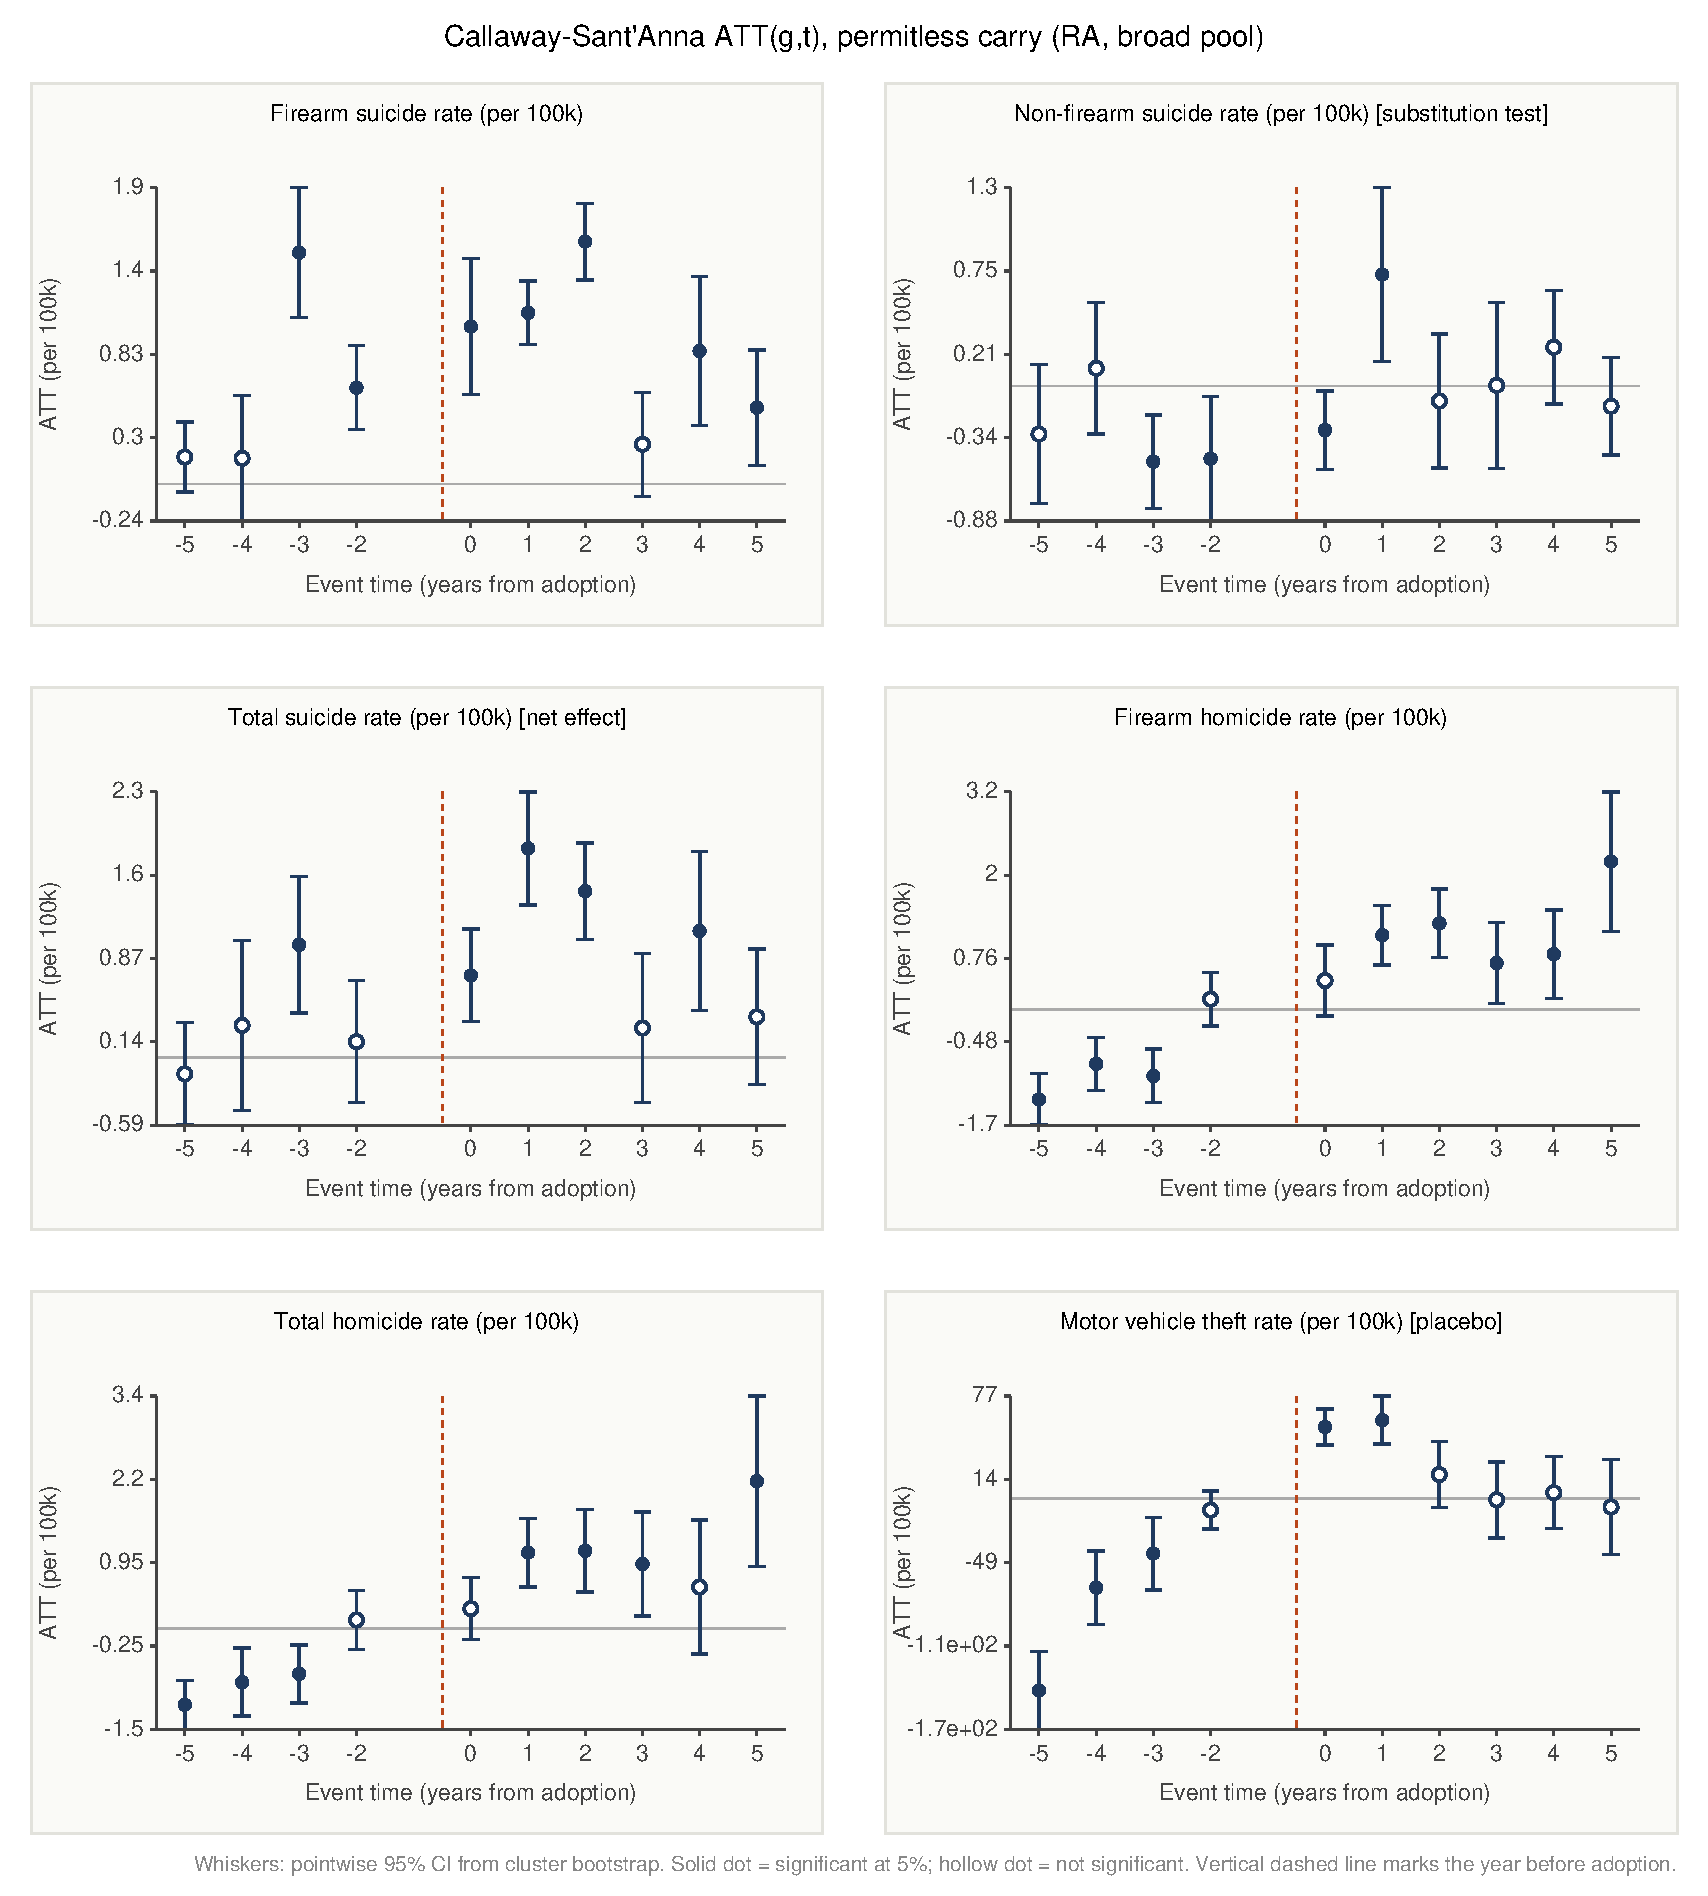
\includegraphics[width=0.95\linewidth]{figures/fig2_cs21_event_study.pdf}
  \caption{Event-study estimates of permitless carry's effect on firearm suicide, by years since adoption.}
  \label{fig:cs21_es}
  \begin{minipage}{0.95\linewidth}\footnotesize
  Estimates from the \citet{callaway2021} event-study estimator,
  with state-cluster wild bootstrap 95-percent confidence intervals
  (two thousand replications). Headline covariate specification;
  never-treated control pool. The dashed vertical line at event
  time $-0.5$ marks the boundary between the pre-policy and
  post-policy periods (year 0 is the year of adoption; year $-1$ is
  the last pre-policy year). Year $-1$ is the reference period: its
  coefficient is normalized to zero by construction and is omitted
  from the plot.
  \end{minipage}
\end{figure}
\bigskip
\begin{figure}[H]
  \centering
  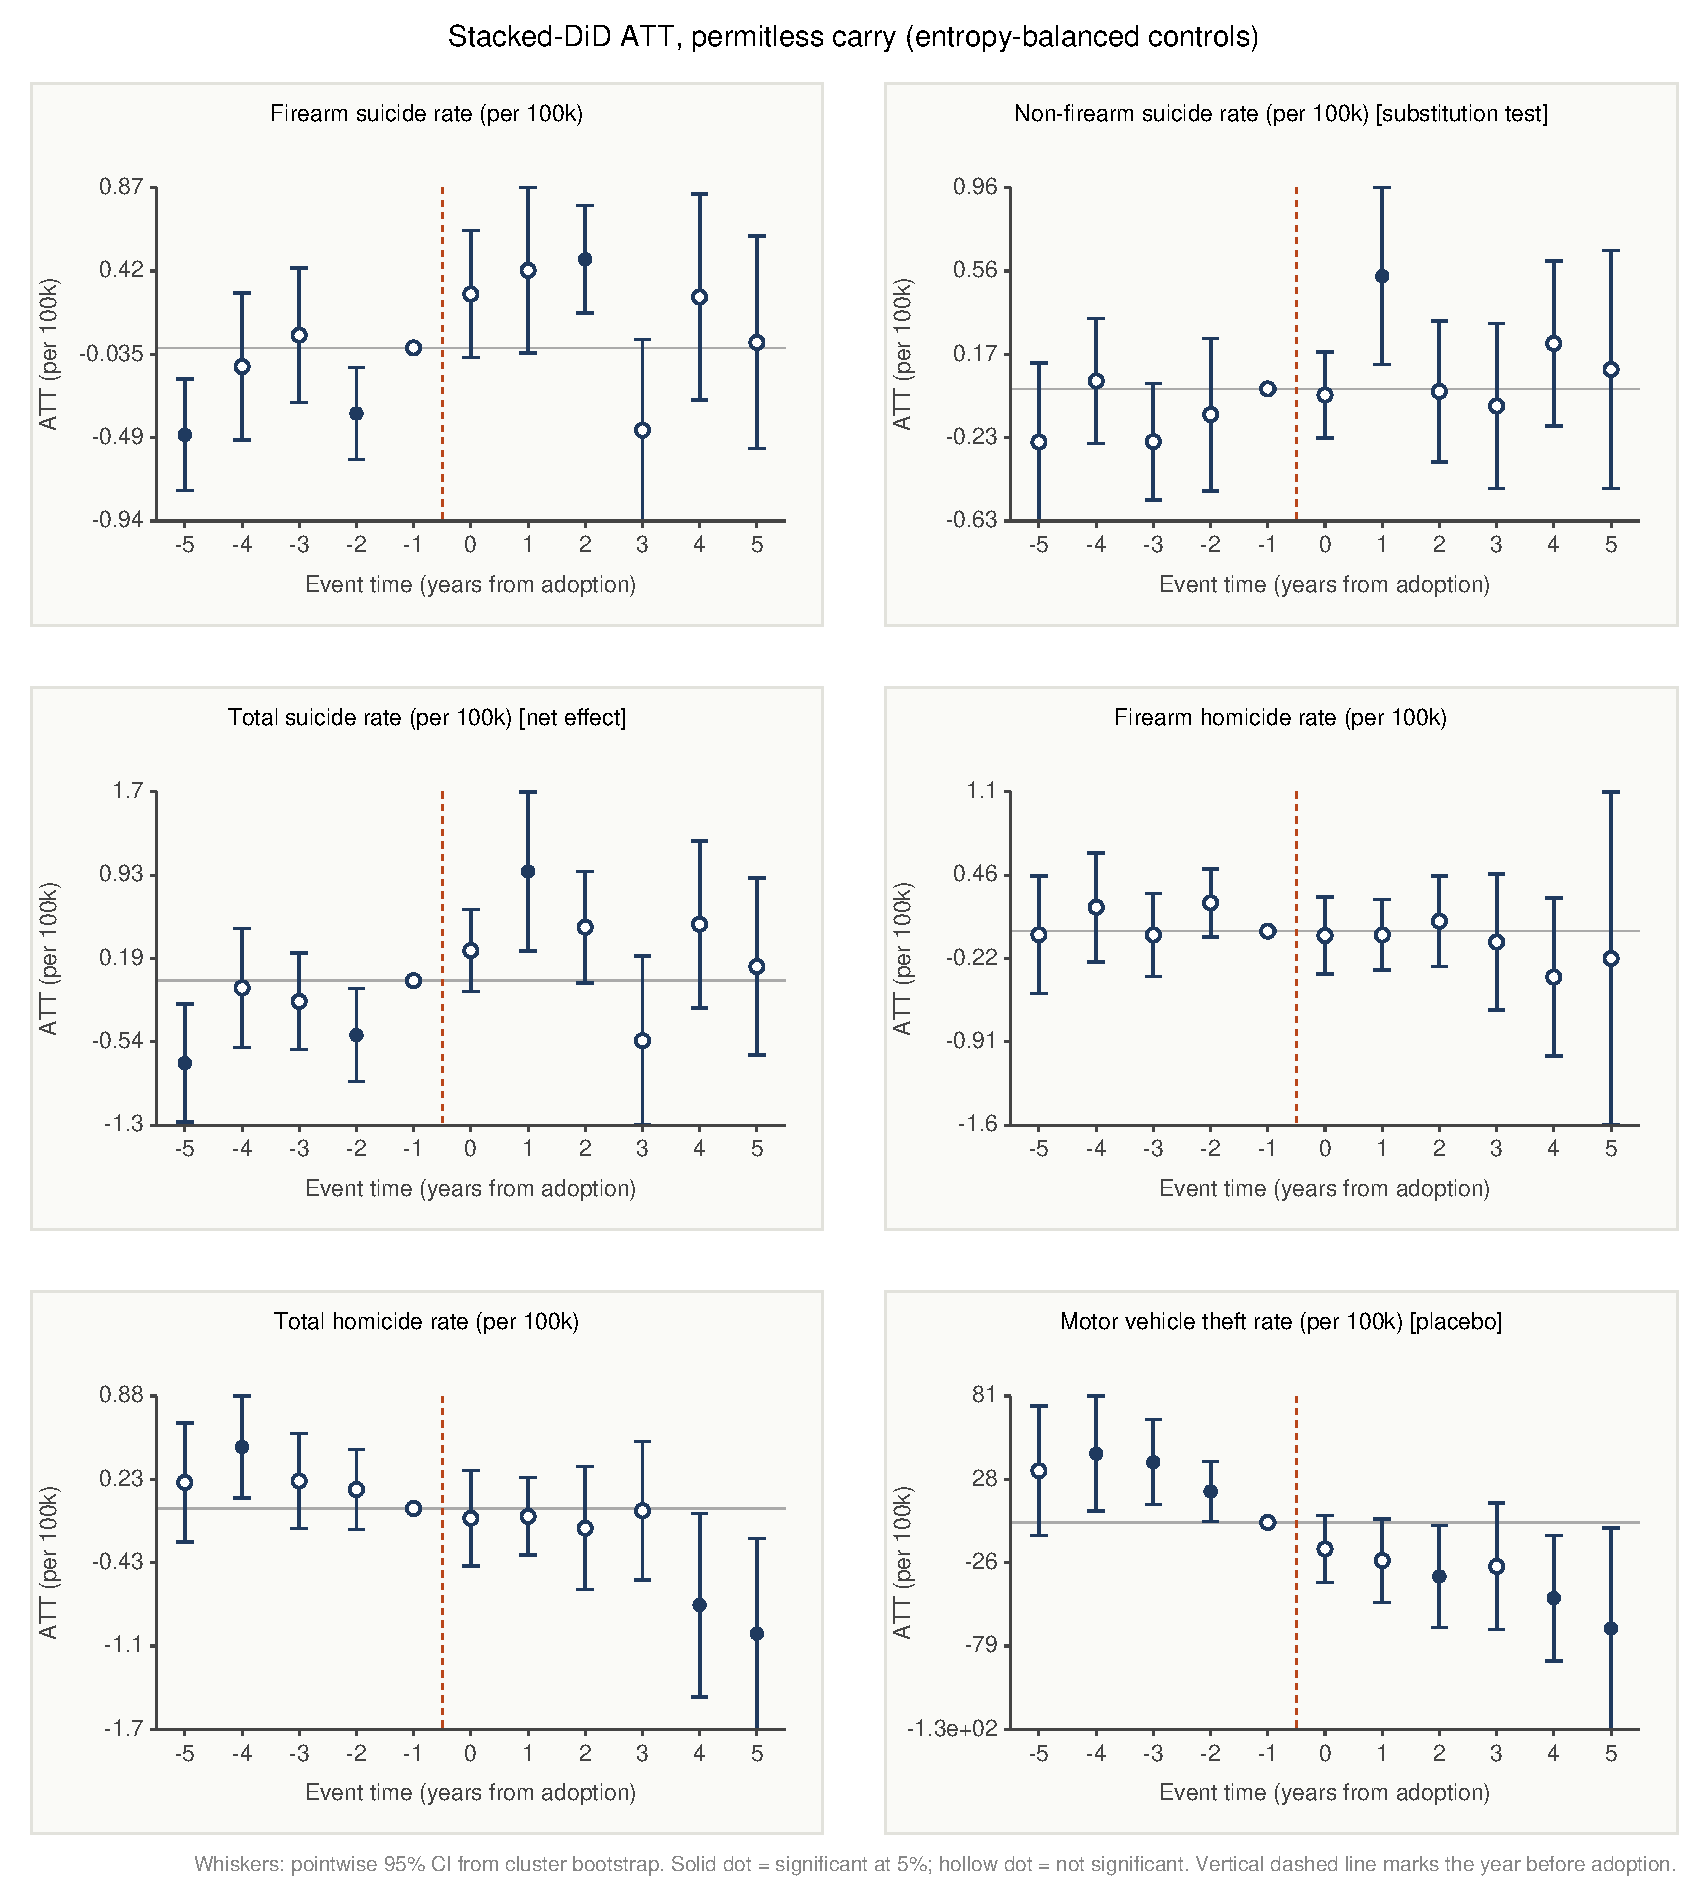
\includegraphics[width=0.95\linewidth]{figures/fig3_stackdd_event_study.pdf}
  \caption{Stacked event-study estimates with entropy balancing, firearm suicide rate.}
  \label{fig:stack_es}
  \begin{minipage}{0.95\linewidth}\footnotesize
  Stacked event-study estimates with state-clustered 95-percent
  confidence intervals. Each adoption cohort contributes a separate
  small panel covering five years before adoption and four years
  after; the never-treated controls in each small panel are
  reweighted via \citet{hainmueller2012} entropy balancing on the
  first and second moments of the headline covariates measured one
  year before adoption. The dashed vertical line at event time
  $-0.5$ marks the boundary between the pre-policy and post-policy
  periods.
  \end{minipage}
\end{figure}
\bigskip
\begin{figure}[H]
  \centering
  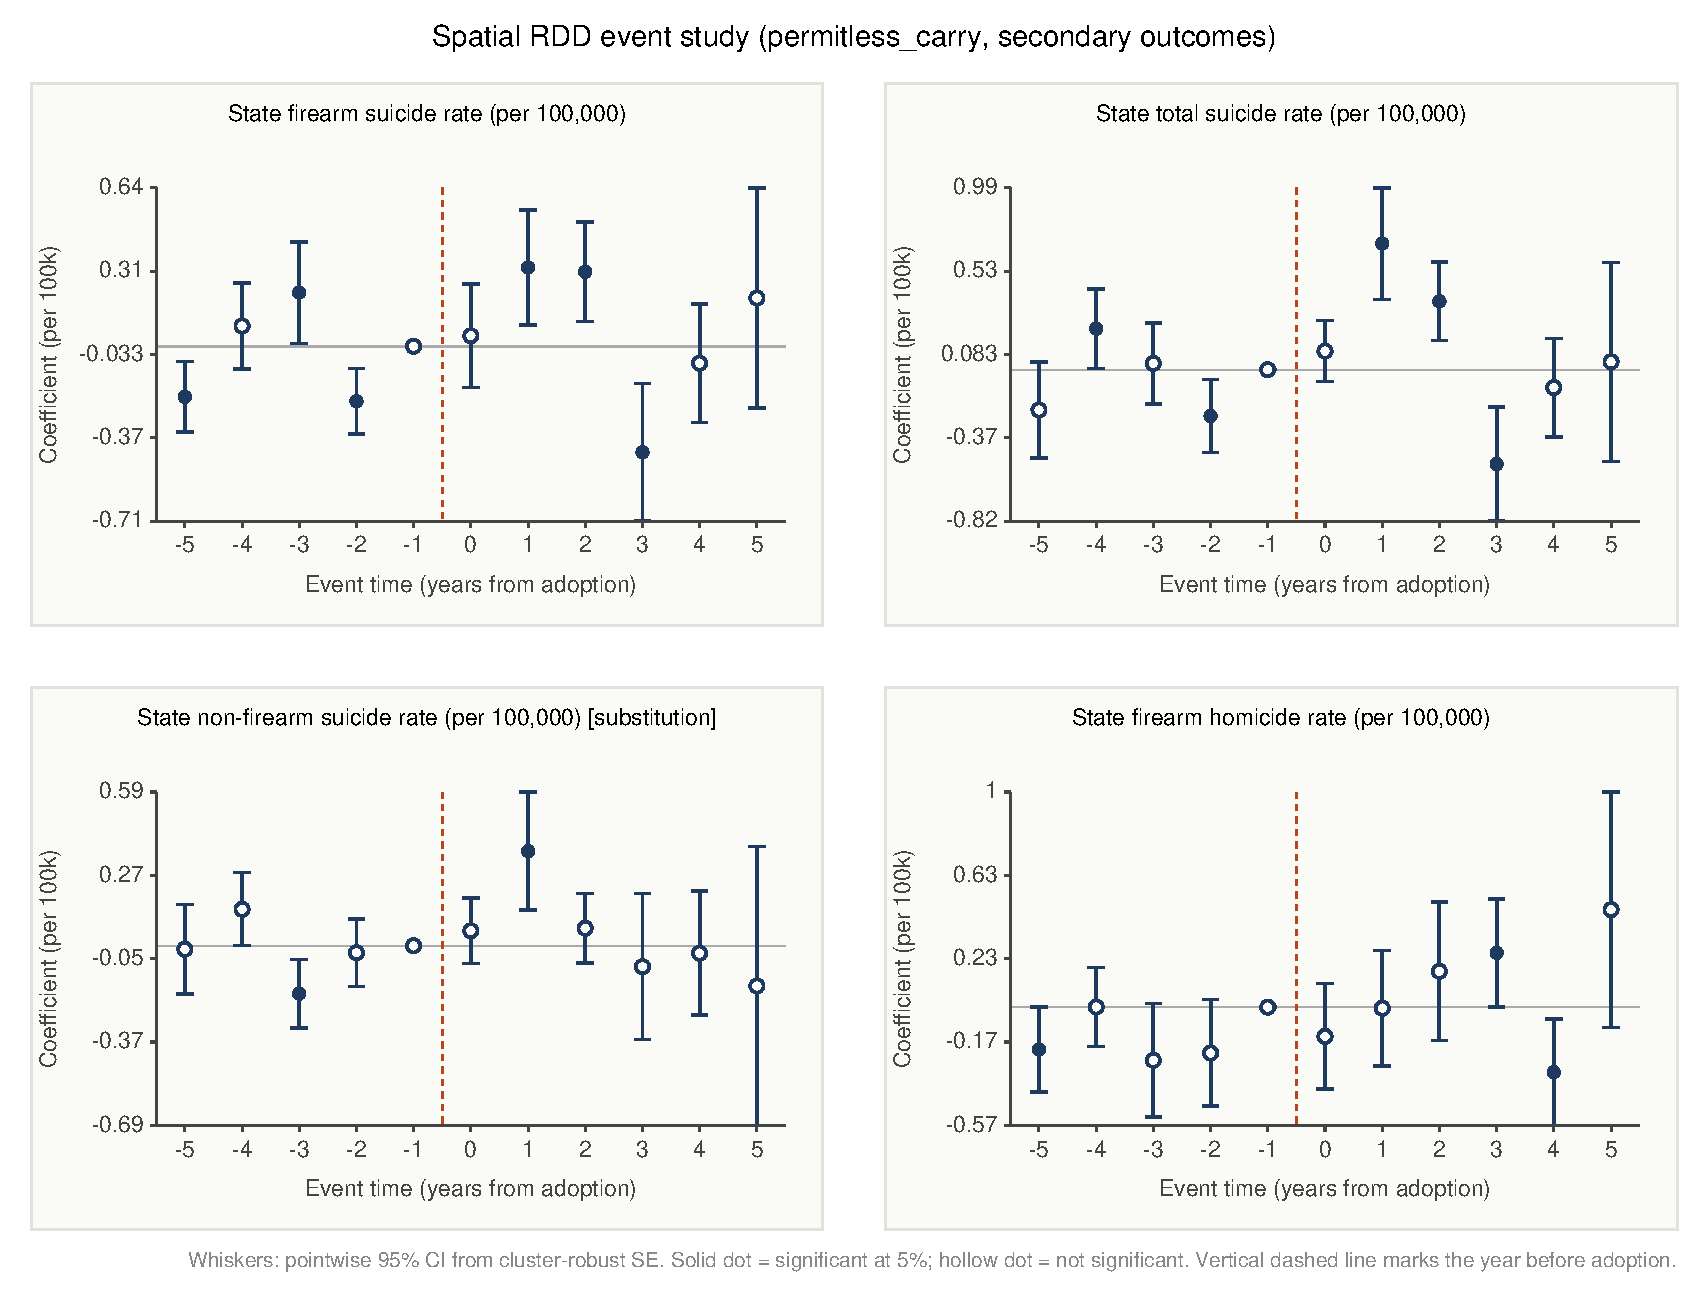
\includegraphics[width=0.95\linewidth]{figures/fig5_rdd_event_study.pdf}
  \caption{Border-county event study: differences within contiguous county pairs straddling a permitless-carry adoption border.}
  \label{fig:rdd_es}
  \begin{minipage}{0.95\linewidth}\footnotesize
  Year-by-year coefficients in a county-panel regression with
  county fixed effects, pair-by-year fixed effects, and the
  headline covariate set. State-clustered 95-percent confidence
  intervals. Bandwidth: 100~km from the adoption border. The
  dashed vertical line at event time $-0.5$ marks the boundary
  between the pre-policy and post-policy periods.
  \end{minipage}
\end{figure}
\bigskip
\begin{figure}[H]
  \centering
  \begin{subfigure}{0.49\linewidth}
    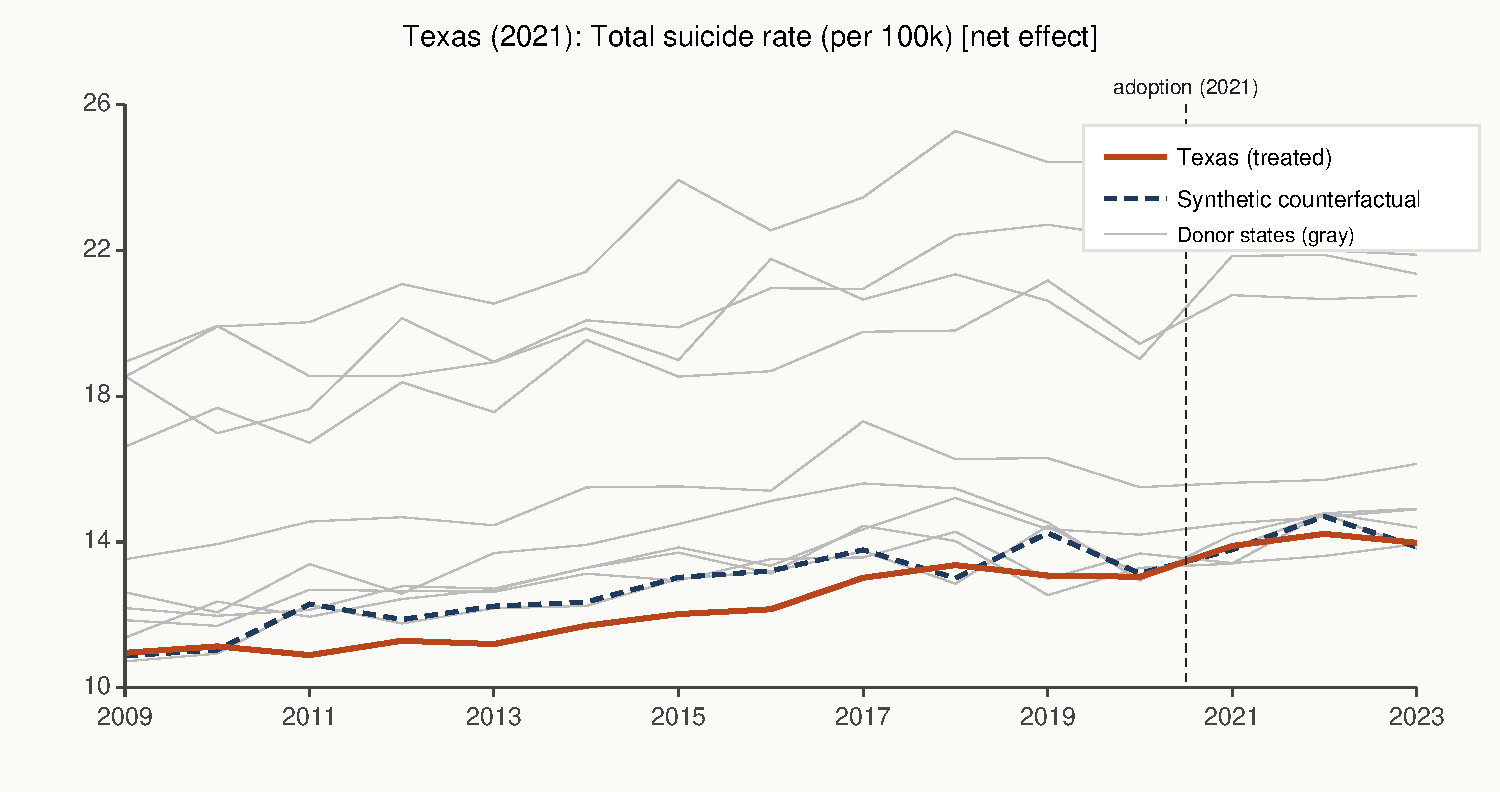
\includegraphics[width=\linewidth]{figures/fig4_scm_TX_2021_total_suicide_rate.pdf}
    \caption{Total suicide.}
  \end{subfigure}
  \begin{subfigure}{0.49\linewidth}
    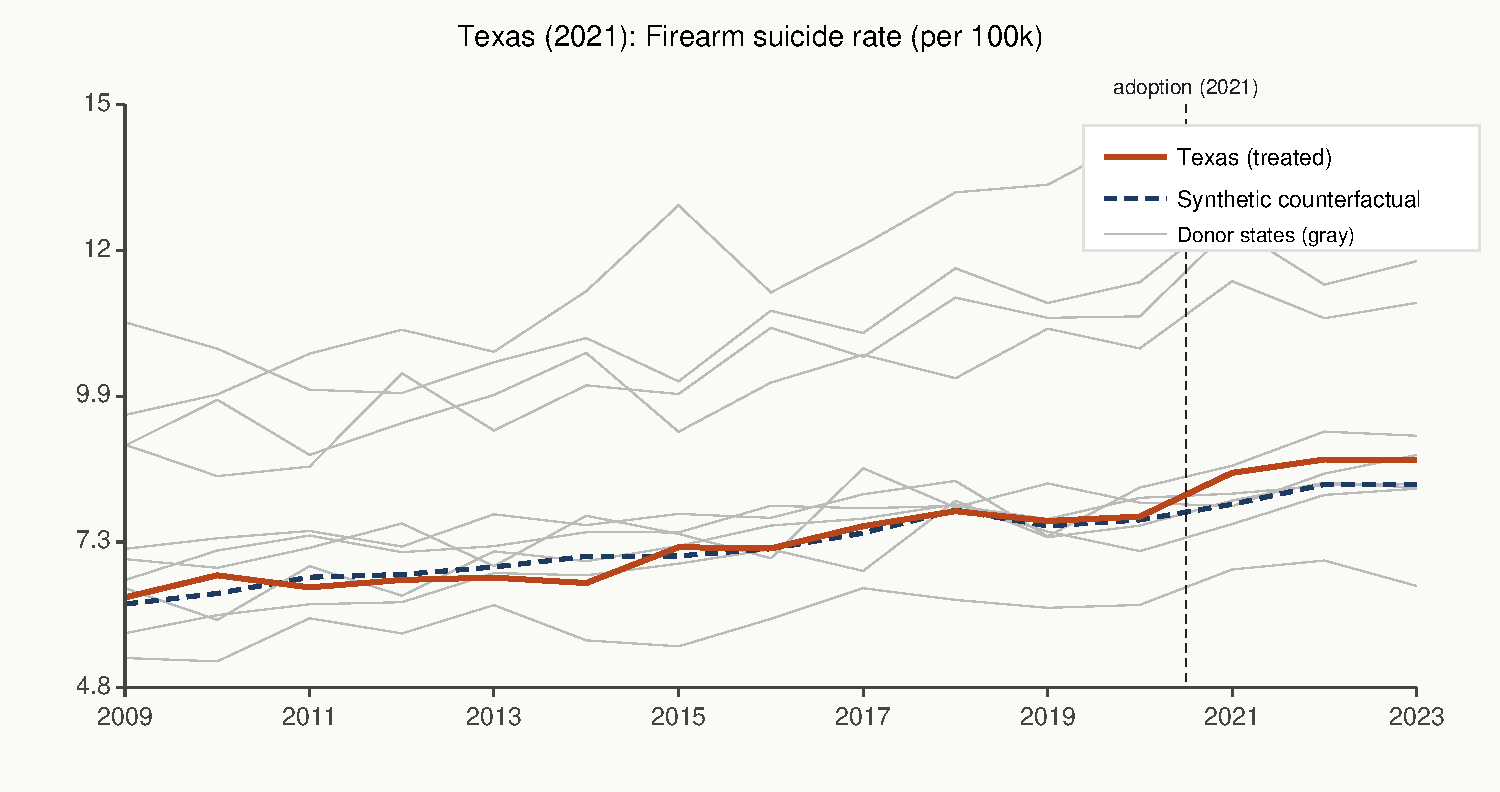
\includegraphics[width=\linewidth]{figures/fig4_scm_TX_2021_firearm_suicide_rate.pdf}
    \caption{Firearm suicide.}
  \end{subfigure}
  \caption{Synthetic-control case study of Texas (2021 adoption).}
  \label{fig:scm}
  \begin{minipage}{0.95\linewidth}\footnotesize
  Texas's actual outcome trajectory (solid) versus its synthetic
  counterfactual (dashed). Donor pool: shall-issue and
  permit-required states throughout the case window. Predictors:
  headline covariate set plus pre-treatment outcome lags.
  \end{minipage}
\end{figure}

\end{document}
